% ************************************************************************** %
% Copyright (C)  2016  Philipp Hacker.																			 %
% Permission is granted to copy, distribute and/or modify this document			 %
% under the terms of the GNU Free Documentation License, Version 1.3				 %
% or any later version published by the Free Software Foundation;						 %
% with no Invariant Sections, no Front-Cover Texts, and no Back-Cover Texts. %
% The lincense itself can be found at <https://www.gnu.org/licenses>.        % 
% ************************************************************************** %

%LICENSE:
%CC BY-NC-SA 3.0 (http://creativecommons.org/licenses/by-nc-sa/3.0/)

% Masters Thesis 
% LaTeX Template
% Version 2.3 (25/3/16)

% This template has been downloaded from:
% http://www.LaTeXTemplates.com

% Version 2.x major modifications by:
% Vel (vel@latextemplates.com)

% This template is based on a template by:
% Steve Gunn (http://users.ecs.soton.ac.uk/srg/
%						  softwaretools/document/templates/)
% Sunil Patel (http://www.sunilpatel.co.uk/thesis-template/)

% ************************************************************************** %
% ************************************************************************** %

% START OF TEX
\documentclass[
	10pt,
	twoside,
	chapterinoneline,
	onehalfspacing, % alternatives: onehalfspacing or doublespacing
	nolistspacing, % If the document is onehalfspacing or doublespacing,
								 % uncomment this to set spacing in lists to single
	%liststotoc, % Uncomment to add the list of figures/tables/etc to toc
	%toctotoc, % Uncomment to add the main table of contents to the toc
	parskip, % Uncomment to add space between paragraphs
	headsepline, % Uncomment to get a line under the header
	english,
]{MastersDoctoralThesis} % The class file specifying the document structure

% ************************************************************************** %
% CORE USEPACKAGE HERE
\usepackage{lmodern}
\usepackage[utf8]{inputenc} % Required for inputting international characters
\usepackage[T1]{fontenc} % Output font encoding for international characters
\usepackage[autostyle=true]{csquotes}
% Required to generate language-dependent quotes in the bibliography
%\usepackage[backend=bibtex,style=authoryear,natbib=true]{biblatex}
\usepackage[backend=bibtex,natbib=true]{biblatex}
% Use the bibtex backend with the authoryear citation style
\addbibresource{bibcontents/preamble.bib} % The filename of the bibliography
\addbibresource{bibcontents/master.bib} % The filename of the bibliography
% ************************************************************************** %

% ************************************************************************** %
% MARGIN
\geometry{%
	% showframe, % show how the type block is set on the page
	paper=a4paper, % Change to letterpaper for US letter
	inner=2cm, % Inner margin
	outer=3.0cm, % Outer margin
	bindingoffset=1.5cm, % Binding offset
	top=1.5cm, % Top margin
	bottom=1.5cm } % Bottom margin
% ************************************************************************** %

% ************************************************************************** %
% THESIS INFORMATION
\date{\today} 
\thesistitle{Kinetic\ effects\ in\ RF\ discharges}
% Your thesis title, this is used in the title and abstract
\supervisor{Prof.\ Dr.\ Ralf\ Schneider}
% Your supervisor's name, this is used in the title page
\examiner{Prof.\ Dr.\ Jürgen\ Meichsner}
% Your examiner's name, this is not currently used anywhere in the template
\degree{Master\ of\ Science\ -\ Physics}
% Your degree name, this is used in the title page and abstract
\author{Philipp\ Hacker}
% Your name, this is used in the title page and abstract
\addresses{Karl-Liebknecht-Ring\ 13,\ 17491\ Greifswald}
% Your address, this is not currently used anywhere in the template
\subject{Physics}
% Your subject area, this is not currently used anywhere in the template
\keywords{plasma,\ discharge,\ kinetic,\ effect,\ physics,\ master}
\university{\href{https://www.uni-greifswald.de/en/}%
					 {Ernst-Moritz-Arndt\ University\ of\ Greifswald}}
% Your university's name and URL, this is used in the title page and abstract
\department{\href{https://physik.uni-greifswald.de/en/}%
					 {Institute\ of\ Physics}}
% Your department's name and URL, this is used in the title page and abstract
\group{\href{https://physik.uni-greifswald.de/ag-schneider/}%
			{Computational\ Sciences}}
% Your research group's name and URL, this is used in the title page
\faculty{\href{https://mnf.uni-greifswald.de/en/faculty/}%
				{Faculty\ of\ Mathematics\ and\ Natural\ Sciences}}
% Your faculty's name and URL, this is used in the title page and abstract
% ************************************************************************** %

\hypersetup{pdftitle=\ttitle} % Set the PDF's title to your title
\hypersetup{pdfauthor=\authorname} % Set the PDF's author to your name
\hypersetup{pdfkeywords=\keywordnames} % Set the PDF's keywords to your keywords

% ************************************************************************** %
% PACKAGES
\usepackage{physics}
\usepackage{mathtools}
\usepackage{amssymb}
\usepackage{upgreek}
\usepackage{esint}
\usepackage{ziffer}
\usepackage{csquotes}
\usepackage{sectsty}
\usepackage{nomencl}

%% FIGURE PACKAGES
\usepackage{float}
\usepackage{graphicx}
\usepackage{subcaption}
\usepackage{wrapfig}
\usepackage{epsfig}

%\usepackage{amsmath}
% cant use svg so easily with subcaption
% \expandafter\def\csname ver@subfig.sty\endcsname{}
% \usepackage{svg}
% ************************************************************************** %

\usepackage{titlesec}
\titleformat{\chapter}[display]
	{\normalfont\huge\bfseries}{}{0pt}{\Huge}
	\titlespacing*{\chapter} {0pt}{20pt}{40pt}

\newcommand{\diff}{\textnormal{d}}
\newcommand{\tenpo}[1]{10^{#1}}
\newcommand{\greek}[1]{\greektext#1\latintext}
\newcommand{\ix}[1]{_\text{#1}}
\newcommand{\imag}{\mathbf{i}}
\newcommand{\tilt}[1]{\textit{#1}}
\newcommand{\divergenz}[1]{\textit{div}\left(#1\right)}
\newcommand{\euler}{\mathnormal{e}}
\newcommand{\fett}[1]{\textbf{#1}}
\newcommand{\inexample}{\text{e.g.}}
\newcommand{\kett}{\rangle}

\renewcommand{\bra}{\langle}
\renewcommand{\grad}[1]{\textit{grad}\left(#1\right)}

% Used for signature line at 
% declaration of authorship
\newcommand{\sign}[1]{%
  \begin{tabular}[t]{@{}c@{}}
  \makebox[1.5in]{\dotfill}\\
  \strut\emph{#1}\strut%
  \end{tabular}%
}

\setlength{\parindent}{0pt}
\setlength{\nomlabelwidth}{.20\hsize}
\setcounter{chapter}{-1}

\setcounter{secnumdepth}{3}
%\setsecnumdepth{subsubsection}

% DOCUMENT START
\begin{document}
%
% ************************************************ %
% RENEWCOMMANDS																		 % 
\renewcommand{\equationautorefname}{equation}			 %
\renewcommand{\figureautorefname}{figure}				   %
\renewcommand{\tableautorefname}{table} 					 %
\renewcommand{\sectionautorefname}{section}				 %
\renewcommand{\subsectionautorefname}{section}		 %
\renewcommand{\subsubsectionautorefname}{section}	 %
\renewcommand{\figurename}{\bfseries Figure}			 %
\renewcommand{\tablename}{\bfseries Table}				 %
\renewcommand{\nomlabel}[1]{#1 \dotfill}					 %
\setlength{\abovedisplayskip}{9pt}                 %
\setlength{\belowdisplayskip}{9pt}                 %
\setlength{\abovedisplayshortskip}{9pt}            %   
\setlength{\belowdisplayshortskip}{9pt}            %
% ************************************************ %
%	
	\frontmatter
  % Use roman page numbering style (i, ii, iii, iv...)
	% for the pre-content pages
	\pagestyle{plain}
  % Default to the plain heading style until the thesis style
	% is called for the body content
%
% TITLEPAGE
\begin{titlepage}
	\begin{center}
		{\scshape\LARGE \univname\par}\vspace{1.5cm} % University name
		% TODO: THESIS TYPE
		\textsc{\Large Master Thesis}\\[0.5cm]
		\HRule\\[0.4cm] % Horizontal line
		{\huge \bfseries \ttitle\par}\vspace{0.4cm} % Thesis title
		\HRule\\[1.5cm] % Horizontal line
		\begin{minipage}[htbp]{0.4\textwidth}
			\begin{flushleft}\large
				\emph{Author:}\\
				\authorname% TODO: AUTHOR NAME
			\end{flushleft}
		\end{minipage}
		\hfill
		\begin{minipage}[htbp]{0.4\textwidth}
			\begin{flushright}\large
				\emph{Supervisor:}\\
				\supname% TODO: SUPERVISOR
			\end{flushright}
		\end{minipage}\\[0.5cm]
		% TODO: UNIVERSITY TEXT
		\large \textit{A thesis submitted in fulfillment of
									 the requirements\\ for the degree of
									 \degreename}\\[0.3cm]
		\textit{in the research group of}\\[0.4cm]
		% TODO: RESEARCH GROUP/DEPARTMENT
		\groupname,\\\deptname\\[1cm]
		%
		% University/department logo - uncomment to place it
		% use for pdf files
		% 
\includegraphics[width=0.50\textwidth]{figures/logos/logo_color.pdf}\\[1.0cm]
		% 
\includegraphics[width=0.55\textwidth]{figures/logos/logo.pdf}\\[1.0cm]
		%
		% use for eps files
		\hspace*{0.75cm}
		
\epsfig{width=0.45\textwidth,file=figures/logos/logo.eps}\\[1.0cm]
		%
		{\large \today} % Date
		\vfill
	\end{center}
\end{titlepage}
%
% ************************************************************************** %
% ACKNOWLEDGMENTS
	 \begin{acknowledgements}
	
		\addchaptertocentry{\acknowledgementname}
		The acknowledgments and the people to thank go here, don't forget to
	 	include your project advisor\ldots
	
	 \end{acknowledgements}
% ************************************************************************** %
%
% ************************************************************************** %
% INSERT MOTIVATIONAL QUOTE
	\vspace*{0.33\textheight}
	% \rule{\textwidth}{0.1pt}
	%	
	\noindent\enquote{%
		Without encroaching upon grounds appertaining to the theologian and the
		philosopher, the domain of natural sciences is surely broad enough to
		satisfy the wildest ambition of its devotees. $\left[\dots\right]$
		The work may be hard, and the discipline severe; but the interest never
		fails, and great is the privilege of achievement.
	}\bigbreak%
	%
	\begin{flushright}
		--- John William Strutt, 3rd Baron Rayleigh, 1884\\
		\small\emph{in: Address to the British Association in Montreal}
	\end{flushright}
	%
	% \vspace*{0.15\textheight}
	% \rule{\textwidth}{0.1pt}
% ************************************************************************** %
%
% ************************************************************************** %
% DECLARATION OF AUTHORSHIP
	%
	\chapter*{Declaration of Authorship}
		%
		I hereby certify that this thesis has been composed by me and is based on 
		my own work, unless stated otherwise.	No other person’s work has been used
		without due acknowledgement in this thesis.
		All references and verbatim extracts have been quoted, and iall sources of
		information, including graphs and data sets, have been specifically
		acknowledged.\\[2.0cm]
		%
		\begin{flushright}
			\sign{Signature of author}\\
			Greifswald; \today
		\end{flushright}
		%
% ************************************************************************** %
%
% ************************************************************************** %
%  TOCTOCTOC FOR EVERYTHING
	\tableofcontents % Prints the main table of contents
	% \listoffigures % Prints the list of figures
	% \listoftables % Prints the list of tables
% ************************************************************************** %
%
% ************************************************************************** %
% PREFIX
	% ************************************************************************** %
% INSERT ABBREVIATIONS
	\begin{abbreviations}{ll}
		\toprule
		\bfseries abbreviation & \bfseries full expression \\%
		\toprule \midrule \endhead%
		e.g.                      & exempli gratia; \emph{for example} \\ \\%
		etc.                      & et cetera; \emph{and so on} \\ \\%
    ac                        & alternating current \\ \\%
    dc                        & direct current \\ \\%
		rf, RF                    & radio frequency \\ \\%
    ccrf                      & capacitively coupled radio frequency \\ \\%
    EDF                       & energy distribution function \\ \\%
		EDV                       & \emph{german: Energieverteilungsfunktion}, energy distribution function \\ \\%
    EEDF                      & electron energy distribution function \\ \\%
    IEDF                      & ion energy distribution function \\ \\%
		p., pp.										& page, plural pages \\ \\%
		ff.												& folio; \emph{on the (next) page}, ablative of folium (\emph{page}) \\ \\%
		HWA												& hard wall approximation \\ \\%
		MS												& mass spectrometer \\ \\%
		PROES											& phase resolved emission spectroscopy \\ \\%
		MWI												& microwave interferometer \\ \\%
		AN												& antenna \\ \\%
		FC												& flow controller \\ \\%
		PIC												& particle-in-cell \\ \\%
		MCC												& Monte-Carlo-Colissions \\ \\%
		
		\midrule \bottomrule
    \caption{%
      List of abbreviations and their corresponding phrases. If specified, the translation %
      or an equivalent expression is written.}\label{tabe:abbreviations}
	\end{abbreviations}
% ************************************************************************** %

% ************************************************************************** %
% CONSTANTS AND SYMBOLS LIST
	\begin{constants}{lcccl}
		\toprule
		\bfseries Quantity & \bfseries Unit &
		\bfseries Symbol & \bfseries Dimension & \bfseries Value \\%
		\toprule \midrule \endhead%
			Speed of Light           & $\unit{m/s}$ & $c\ix{0}$ & $\unit{L^{1}T^{-1}}$ & $2,997\cdot\tenpo{8}$ \\ \\%
      thermal velocity         & $\unit{m/s}$ & $v\ix{th,j}$ & $\unit{L^{1}T^{-1}}$ & \\ \\%
      drift velocity           & $\unit{m/s}$ & $v\ix{D,j}$, $u\ix{j}$ & $\unit{L^{1}T^{-1}}$ & \\ \\%
      Boltzmann constant       & $\unit{eV/K}$ & $k\ix{B}$ & $\unit{M^{1}L^{2}T^{-2}K^{-1}}$ & $8,617\cdot\tenpo{-23}$ \\ \\%
      mobility                 & $\unit{cm^{2}/Vs}$ & $\mu\ix{j}$ & $\unit{I^{1}T^{2}M^{-1}}$ & \\ \\%
			planck constant          & $\unit{eVs}$ & $\hbar$ & $\unit{G^{-1/2}c^{6/2}\varepsilon\ix{0}^{1/2}}$%
                                                        & $\unit[4,1345\cdot\tenpo{-15}]{eVs}$ \\ 
															 & & & & $\unit[6,646\cdot\tenpo{-34}]{Js}$ \\ \\%
			kinetic temperature      & $\unit{eV}$ & $T\ix{j}$ & $\unit{M^{1}L^{2}T^{-2}}$%
                                                         & $\unit[1]{eV}=\unit[1,902\cdot\tenpo{-19}]{K}$ \\ \\%
			elementary charge        & $\unit{C}$ & $e$ & $\unit{I^{1}T^{1}}$ & $1,902\cdot\tenpo{-19}$ \\ \\%
      electric charge          & $\unit{C}$ & $Q$, $q$ & $\unit{I^{1}T^{1}}$ & \\ \\%
      particle mass            & $\unit{kg}$ & $m\ix{j}$ & $\unit{M^{1}}$ & electron: $9,109\cdot\tenpo{-31}$ \\
                               &	&	& & \hspace*{.65cm} ion: $5,310\cdot\tenpo{-26}$ \\
                               &	&	& & \hspace*{.3cm} anion: $5,143\cdot\tenpo{-26}$ \\ \\%
			reduced mass             & $\unit{kg}$ & $\mu\ix{j,k}$ & $\unit{M^{1}}$ & \\ \\%
      distance,location        & $\unit{cm}$ & $r$, $\vec{r}$ & $\unit{L^{1}}$ & \\ \\%
			Debye length             & $\unit{cm}$ & $\lambda\ix{D,j}$ & $\unit{L^{1}}$ & \\ \\%
			particle distance        & $\unit{cm}$ & $\overline{b}$ & $\unit{L^{1}}$ & \\ \\%
			mean free path           & $\unit{cm}$ & $s\ix{mfp,j}$ & $\unit{L^{1}}$ & \\ \\%
      particle density         & $\unit{cm^{-3}}$ & $n\ix{j}$ & $\unit{L^{-3}}$ & \\ \\%
      Vacuum permittivity      & $\unit{F/m}$ & $\varepsilon\ix{0}$%
                                              & $\unit{M^{-1}L^{-3}T^{-4}A^{2}}$ & $8,854\cdot\tenpo{-12}$ \\ \\%
			electrostatic potential  & $\unit{V}$ & $\Phi$, $U$ & $\unit{M^{1}L^{2}I^{-1}T^{-3}}$ & \\ \\%
      electric current         & $\unit{As}$ & $I$, $J$ & $\unit{I^{1}}$ & \\ \\%
      electric current density & $\unit{As/cm^{2}}$ & $j\ix{j}$ & $\unit{I^{1}L^{-2}}$ & \\ \\%
      electric charge density  & $\unit{C/cm^{3}}$ & $\rho$ & $\unit{I^{1}T^{1}L^{-3}}$ & \\ \\%
    \midrule\bottomrule% pagebreak
      electric resistance      & $\unit{\Omega}$ & $R$ & $\unit{M^{1}L^{2}T^{-3}I^{-2}}$ & \\ \\%
      electric capacity        & $\unit{F}$ & $C$ & $\unit{M^{-1}L^{-2}T^{4}I^{2}}$ & \\ \\%
      time                     & $\unit{s}$ & $t$ & $\unit{T^{1}}$ & \\ \\%
      plasma frequency         & $\unit{Hz}$ & $\omega\ix{p,j}$ & $\unit{T^{-1}}$ & \\ \\%
      collisional frequency    & $\unit{Hz}$ & $\nu\ix{j}$ & $\unit{T^{-1}}$ & \\ \\%

		\midrule\bottomrule
    \caption{%
      Physical properties in their commonly --- or for this purpose most convinient %
      --- units and corresponding SI units. If not specified, the values of each quantity %
      refer to the afore-mentioned units.}\label{tabe:physicalconstants}
	\end{constants}
% ************************************************************************** %


% ************************************************************************** %
\mainmatter% Begin numeric (1,2,3...) page numbering
\pagestyle{thesis} % Return the page headers back to the "thesis" style
% ************************************************************************** %
% INSERT ABSTRACT
 	% 
	\chapter{Abstract}
		%
    The Thesis Abstract is written here and usually kept to just this page.
    The page is kept centered vertically so it can expand into the blank space above 
    the title too.
  	%
% ************************************************************************** %
% BASICS
	%
\chapter{Physical Properties of Low Temperature RF Plasma}\label{sec:chapter_ccrfbasics}
%
	In this first chapter I will provide the necessary physical background for this work about the numerical simulation of low temperature capacitively coupled radio frequency plasma. Here both the mathematical basics and method for the simulation, as well as the most important aspects about the plasma properties will be explained.
%
	\section{Plasma Physics}\label{sec:plasmaphysics}
%
  	\subsection{Capacitively Coupled Radio Frequency Plasma}\label{sec:ccrf}
%
		The experiment where after the conducted simulations is modelled after revolves around a capacitively coupled radio frequency, low temperature plasma at low pressures of oxygen. Here, I will refer to a plasma as an globally quasi-neutral gas, consisting of freely moving charges --- e.g.\@ electrons, positively and negatively ions --- and neutral gas particles. The ratio between charged and neutral species defines the \emph{degree of ionization}, which in this case is very low. The term of global neutrality emphasizes the purpose for different length scales inside the gas itself. Hence, the associated condition of neutrality by equal densities $n\ix{e}\,=\,n\ix{i}$ only is valid for areas larger than the so called \emph{Debye sphere}. Inside this ball with a radius of $\lambda\ix{D}$ the \emph{Debye length}, the afore-mentioned neutrality is not satisfied.\\
		The creation of a plasma is accomplished by 2 parallel metal plates, the electrodes, where on at least one an ac signal at radio frequency is applied --- this kind of experimental setup is among the most common, thus being used for basic but also in-depth studies of the afore-mentioned discharges. Here, a rf signal at exactly $\unit[13,56]{MHz}$ with an amplitude between $100$--$\unit[1000]{V}$ will be used. This equals to a wavelength of $\unit[22,11]{m}$ for the electric field wave, which is orders of magnitude higher than the eventually simulated experiment. The use of external magnetic fields is not within the scope of this work --- correspondingly, the experiment I will refer to, also did not include any kinds of magnetic confinement or manipulation. \\
		That said, a multitude of electric setups are possible, such as coated or grounded electrodes. Therefore, different regimes of operation ensue. For example, differently driven or shaped metal plates heavily influence the charge creation process inside the plasma. In summary, the electrodes, neutral gas and electric layout resemble a dielectric hindered plate capacitor.
%
		\begin{wrapfigure}{r}{0.42\textwidth}
			\centering
			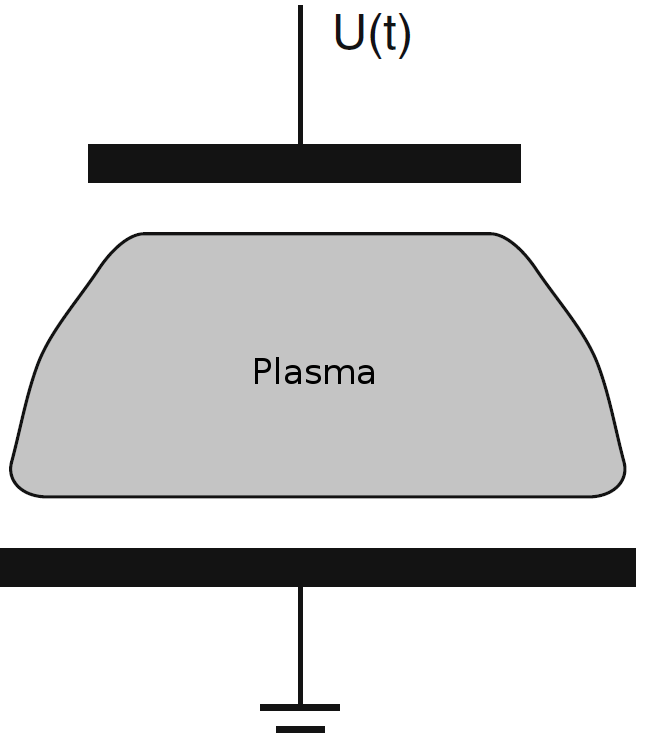
\includegraphics[width=0.38\textwidth]{figures/circuitselfbias_1.png}
			\caption{%
				Schematic of an asymmetric discharge with one grounded and one driven electrode.%
			The rf signal is denoted with $U(t)$.~\cite{Piel10}}\label{fig:circuitselfbias_1}
		\end{wrapfigure}
%
		This simplification can be used to access important physical properties, such as an additional voltage offset on one of the electrodes or charge currents at such. A basic scheme of an asymmetric rf discharge can be seen in~\autoref{fig:circuitselfbias_1}. In the case of different electrode sizes, as seen in the scheme, the potential inside the spatially restricted area between wall and discharge can change drastically. This plasma sheath forms also between grounded parts of discharge containment or probes and plasma volume. This additional direct current offset is called \emph{self-bias} (see~\autoref{sec:selfbias}). A dielectric displacement current between plasma sheath and volume accommodates as a result of the different time scales of particle movement (see~\autoref{sec:displacementcurrent}). Especially, self-bias and displacement current play a key role in the following investigations, as a capacitive coupling between electrodes and power supply is difficult to model in a numerical kinetic simulation.\\
		A strong mathematical analysis of general plasma properties would not be suitable for this kind of work, although certain aspects will be discussed later, such as in~\autoref{sec:selfbias} and~\autoref{sec:displacementcurrent}.
		In comparison to other low temperature, low pressure discharges  --- an example could be a dielectric hindered dc discharge at high voltages, with an electrode space gap of just a couple millimeters ---, radio frequency plasma are characterized by their unique transport process inside the sheath and heating mechanisms of charged species. A more in-depth discussion can be found in~\autoref{sec:heating}.\\ 
%
		\subsection{Plasma-Wall Interaction}\label{sec:sheathphysics}
%
			In the discharges bulk, neutral gas particles are excited by electron collisions and radiating visible light. However, areas around, e.g.\@ floating metal surfaces, probes and grounded walls are darker than the bulk. This is due to the low electron density and kinetic energy in this \emph{plasma sheath}. Though areas with vanishing electron numbers can glow because of high collision efficiencies and/or frequencies.\\
			Electrons, in general, are of a much higher mobility $\mu\ix{e}$ and thermal velocity $v\ix{th,e}$. Hence they impinge onto walls and surfaces more often than other species, leading to a --- in this case we consider an electronegative oxygen discharge, where the following can be assumed true --- negative charge and potential.
%
			\subsubsection{Child-Langmuir Law}\label{sec:langmuirlaw}
%
				For an asymmetric ccrf discharge, dc \emph{self bias} and displacement current are important parts of the electric system. Hence, the \emph{Child-Langmuir Law} as a function of those properties can be written. The rf component of the excitation is neglected.\\
				A greatly negative charged wall at $x=0$ shall be a barrier for electrons of thermal velocity, e.g.\@ $|\Phi(0)-\Phi(d)|\ll k\ix{B}T\ix{e}/e\,$. The thickness of the sheath shall be considered $d$. In an one-dimensional approach~\cite{Piel10}, the electron density $n\ix{e}(x)$ can be written with a \emph{Boltzmann} distribution function $f\ix{B}(\Phi)$:
%
				\begin{align}
					n\ix{e}(x)=n\ix{e}(d)\cdot f\ix{B}(\Phi)=%
					n\ix{e}(d)\cdot%
					\exp{\left(\frac{e{\left(\Phi(x)-%
							\Phi(d)\right)}}{k\ix{B}T\ix{e}}\right)}\quad.%
					\label{equ:electrondens}
				\end{align}
%
				This means that the electron density decreases exponentially towards the negatively charged wall. It can be assumed that the sheath thickness $d\ll s\ix{mfp,i}$ the mean free path of the ions inside the plasma bulk. Hence, ions enter the sheath collisionless.\\
				At the boundary between bulk and pre-sheath, the walls potential vanishes because of the plasmas shielding capabilities. Here, the ions are at $v\ix{i,0}$ speeds, therefore their density becomes:
%
				\begin{align}
					n\ix{i}(x)=n\ix{i}(d){\left(1-\frac{2e\Phi(x)%
							}{m\ix{i}v\ix{i,0}^{2}}\right)}^{-1/2}%
					\label{equ:iondens}
				\end{align}
%
				Futhermore, one can assume that the kinetic energy at this point is smaller than the potential energy for the acceleration inside the pre-sheath, e.g.\@ $m\ix{i}v\ix{i,0}^{2}\ll |e\Phi(x)|$. Using \emph{Poisson's } equation, and taking into account the ion-sheath interaction,~\autoref{equ:phibypoisson} gives an equation for $\Phi(x)$:
%
				\begin{align}
					\Delta\Phi\cong-\frac{en\ix{i}{\left(-d\right)}%
							}{\varepsilon\ix{0}}{\left(-\frac{2e\Phi{%
							\left(x\right)}}{m\ix{i}v\ix{i,0}^2}\right)}^{-\frac{1}{2}}%
					\label{equ:phibypoisson}
				\end{align}
%
				Solving this, and using the unpertubated ion current $j\ix{i}=n\ix{i}(d)ev\ix{i,0}$, one yields the result by \emph{Langmuir}.
%
				\begin{align}
					\Phi{\left(x\right)}={\left({\left(\frac{3}{4}{\left(x+d%
							\right)}\right)}^4{\left(\frac{j\ix{i}}{\varepsilon\ix{0}%
							}\right)}^2\frac{m\ix{i}}{2e}\right)}^{\frac{1}{3}}%
					\label{equ:langmuirpot}
				\end{align}
%
				Again, solving~\autoref{equ:langmuirpot} for the current $j\ix{i}$ yields the \emph{Child-Langmuir Law} (see~\autoref{equ:childlangmuirlaw}).\\
				This equation defines the ion current as a function of the unperturbed plasma bulk. In other words, the sheath changes its thickness in dependency of those certain discharge parameters, always satisfying the ion current defined by the \emph{Child-Langmuir Law}.
%
				\begin{align}
					j\ix{i}=\frac{4}{9}\varepsilon\ix{0}{\left(\frac{2e{%
							\left(\Phi{\left(-d\right)}-\Phi{\left(0\right)}%
							\right)}^3}{m\ix{i}d^2}\right)}^{\frac{1}{2}}%
					\label{equ:childlangmuirlaw}
				\end{align}
%
			\subsubsection{Surface Effects and Secondary Ion Emission}\label{sec:surfaceeffects}
%
				Although plasma sheath physics are influenced by bulk properties, such as temperatures and densities, the space charge area itself is mainly characterized by processes of the wall. Hence an important aspect is the absorption and re-emission of ions and electrons.	Those species than have unique features, like e.g.\@ high velocities. Let's assume the associated metal wall behind the sheath ideally absorbs all impinging, charged particles, which recombine immediately near the surface.\\
%
				\paragraph{Secondary Electron Emission}
				The discharges electrons are much faster and mobile than the other species, leading to the afore-mentioned negative charging and potential drop towards the wall. This accelerates the ion species up to \emph{Bohm velocity} --- see~\autoref{sec:bohmcriteria} for a more in-depth discussion of the \emph{Bohm criteria} and the ions sheath physics.\\
				Continuity and charge conservation must be satisfied, hence the fluxes $J\ix{j}$ of the species $j$ must be equal at the sheath edge --- into and out of the sheath:
%
				\begin{align}
					J\ix{e}=J\ix{i}%
					\label{equ:sheathequi}
				\end{align}
%
				The mentioned potential drop $\Delta\Phi$ from~\autoref{sec:langmuirlaw}, beside accelerating positive ions, reflects negative charges slower than $v\le \sqrt{2e\Delta\Phi/ m}\,$. Similar to~\autoref{equ:electrondens}, the electron current towards the wall can be written. Here the first moment of the electron velocity $\bra v\kett$ is used, calculated in~\autoref{equ:firstmoment} with the electron energy distribution function (EEDF) $f\ix{e}(v)$:
%
				\begin{align}
					j\ix{e}=&-\frac{e}{4}n\ix{e}\bra v\kett\exp\left(-\frac{e\Delta\Phi}{k\ix{B}T\ix{e}}\right)%
					\label{equ:electroncurrent}\\[0.0cm]
					\bra v\kett=&\int_{\mathbb{R}}v\cdot f\ix{e}\left(v\right)\diff v%
					\label{equ:firstmoment}
				\end{align}
%
				Impinging ions are neutralized before impact by particles from the electron gas in the wall. Like before, any produced neutrals are reflected and exit the sheath collisionless --- the mean free path is larger than the sheath thickness. Hence ionization is a process almost exclusively happening in the bulk or the pre-sheath.\\
				Assuming a fast electron impacts on the wall, there is a chance of colliding with and liberating a second electron from the target. Here, the \emph{secondary electron emission} coefficient is noted as $\gamma$: an impinging electron emits $\gamma$-many electrons from the metal. This \emph{SEE} reduces the $\Delta\Phi$ because of an addition charge current from the wall towards the sheath edge, therefore altering the continuity condition $j\ix{i}=j\ix{e}$. A new \emph{effective potential drop} $\Delta\Phi\ix{eff}$ can be written in~\autoref{equ:effectivepotentialdrop}. According to~\cite{} there is a critical value $\gamma\ix{c}$ from which on the wall potential is unstable, leading to shifting sheath edges --- the sheath edge oscillates with the rf signal anyway --- and strong currents from the wall.
%
				\begin{align}
					\Delta\Phi\ix{eff}=-\frac{k\ix{B}T\ix{e}}{e}\cdot\ln\left(\left(1-%
							\gamma\right)\sqrt{\frac{m\ix{i}}{2\pi m\ix{e}}}\,\right)%
					\label{equ:effectivepotentialdrop}
				\end{align}
%
				\paragraph{Secondary Ion Emission}	
				Research prior to this thesis~\cite{Kullig12} indicates that ions are produced near the surface of a metal electrode and heavily accelerated in the plasma sheath. In theory, secondary emission by surface ionization --- in analogy to the surface neutralization --- occurs with incident atoms of thermal energy. Hence one assumes a positively biased wall at high temperatures as the target. It's valence level is therefore broadened, giving an atom $A$ the chance the deposit an electron at the metal. After equilibrating thermally, a positive ion is emited by chance. This statistical process can be described by a thermodynamic equation (see~\autoref{equ:sahalangmuirpos}) yielding the ionization coefficient of $A$. In~\autoref{equ:sahalangmuirpos} a modified approach for the \emph{Saha-Langmuir equation} on the degree of ionization in gases can be found. Here, the surface's temperature $T$ and average work function $\overline{\Phi}_{+}$ are needed. Additionally, the ionization energy $I(A)$ --- or impact energy ---, the particle number currents of both species $j$ and $j^{+}$, corresponding statistical weights $w$, $w^{+}$ and reflection coefficients at the intrinsic potential barrier $r$/$r^{r}$ are used.
%
				\begin{align}
					A\leftrightharpoons A^{+}+&\,e^{-}%
					\label{equ:positiveion}\\[0.0cm]
					\alpha^{+}(A^{+})=\frac{j^{+}}{j}=\frac{(1-r^{+})\,w^{+}}{(1-r)\,w}\cdot&\exp\left(%
					\frac{\overline{\Phi}_{+}+e\sqrt{eV\ix{ext}}-I(A)}{k\ix{B}T}\right)%
					\label{equ:sahalangmuirpos}
				\end{align}
%
				At high temperatures of, e.g.\@ $\unit[1000]{K}$ and externally applied potentials $V\ix{ext}<\unit[1]{kV}$, the reflection associated \emph{Schottky term} $e\sqrt{eV\ix{ext}}$ and the corresponding coefficients $r$/$r^{+}$ can be neglected --- it appears to be just half of the thermal energy at room temperature. Though a theoretical approach is possible, there have not been accurate studies of such coefficients for temperatures around $\unit[300]{K}$.\\
				In addition to SIE of positive ions, a case for negative ions can be easily derived with small changes to~\autoref{equ:sahalangmuirpos}: a negatively biased electrode is assumed and the average work function yields a different sign. The electron affinity of the incident particle $B$ is noted as $A(B)$.
%
				\begin{align}
					B+\,&e^{-}\leftrightharpoons B^{-}%
					\label{equ:negativeion}\\[0.2cm]
					\alpha^{-}(B^{-})=\frac{(1-r^{-})%
						\,w^{-}}{(1-r)\,w}\cdot&\exp\left(%
						\frac{-\overline{\Phi}_{-}+e\sqrt{eV\ix{ext}}+A(B)}{k\ix{B}T}\right)%
					\label{equ:sahalangmuirneg}
				\end{align}
%
				Applying the former assumptions to both equations of positive and negative ions, inserting a homogeneous work function $\Phi=\overline{\Phi}_{-}=\overline{\Phi}\ix{+}$ for the used substrate yields the originally derived \emph{Saha-Langmuir equations}.
%				
				\begin{align}
					\alpha^{+}(A^{+})=\frac{w^{+}}{w}\,\exp\left(\frac{%
					\Phi-I(A)}{k\ix{B}T}\right)\,,%
						\quad\quad%
					\alpha^{-}(B^{-})=\frac{w^{-}}{w}\,\exp\left(\frac{%
						-\Phi+A(B)}{k\ix{B}T}\right)%
						\label{equ:sahalangmuirshort}
				\end{align}
%
				Though only considering atomic particle beams onto the wall until this point, forms similar to~\autoref{equ:sahalangmuirshort} can be derived for molecular surface interactions~\cite{Kawano83}. In case of the earlier discussed ccrf discharges, arguments like high temperatures can not be applied, hence the need for measured reflection coefficients.\\
				Works of, e.g.\@~\cite{Ustaze97} and~\cite{Los90} investigated ion beam scattering, electron loss and transport in plasma sheath environments for metal walls, especially $\text{MgO}(100)$ surfaces. There Ustaze et al.\ studied incident oxygen gas particles --- ions and neutrals ---  on magnesium oxyde surfaces. Impinging atoms became negatively charged ions, picking up electrons from the $\text{MgO}$ of the wall. This interaction, though requiring a minimum ionization and liberation energy for the electron, is most effective at low energies $<\unit[1]{eV}\,$. This is due to a maximum of residence time at the target for an incoming atom. Hence it can be considered a non-resonant charge transfer process at the anion site. For an more in-depth discussion of both electron loss and capture for anion transport processes at walls one should consider~\cite{Kawano83}.\\
				Here, due to the lack of theoretical and experimental data on ion surface production, an ion beam onto the wall will result in a anion current in opposing direction of
%
				\begin{align}
					j_{-}=\eta\,j\ix{+}\,\,,%
					\label{equ:negative_efficiency}
				\end{align}
%
				with a corresponding efficiency of an incident positive particle $\eta\,$. One should keep in mind the reaction of the plasma sheath and potential inside to an additional anion current from the wall. Also, the same stability criteria apply for $\eta$ as they do for the electron emission coefficient $\gamma$. In case of SIE beyond a critical value $\eta\ix{c}$, a second plasma sheath may develop, enclosing the bulk and an inner sheath and reducing transport in-between.

	%
		\subsection{Bohm Criteria}\label{sec:bohmcriteria}
%
			In~\autoref{sec:sheathphysics} the behaviour of charge particle densities inside the plasma sheath has been discussed. In contrast to the discharge volume, those densities do not satisfy the quasi-neutrality condition in a distance of $d$ from the wall any more. Though we know that the sheath is a spatially restricted area around electrostatic floating surfaces, a physical law concerning this circumstance has not been derived here. So the question ensues, why the area of electron depletion does not extend further into the discharge volume.\\
			To answer this question, one has to take a look at a substitutional system. This will be a, likewise mechanical, one-body extremal problem of a point mass. In this case only kinematic potentials with inverted parabolic maxima are of interest. Therefore, in this unstable equilibrium, a small pertubation culminates into a large force on the test body.\\
			To see the quality of this example, one has to take a look at the second order differential equation of the afore-mentioned mechanical problem and the electrostatic \emph{Poisson's equation} (see~\autoref{equ:pseudo}).
%
			\begin{align} 
				m\frac{\diff^{2}\vec{r}}{\diff t^{2}}=-\frac{\diff V}{\diff\vec{r}}%
						\quad\Leftrightarrow\quad%
						\Delta_{\vec{r}}\Phi=-\frac{\diff\Psi}{\diff\Phi}=f{\left(\Phi\right)}%
						\hspace{-0.33cm}\overset{\text{Poisson's}}{\overset{\mid}{=}}\hspace{-0.33cm}%
						\frac{\rho}{\varepsilon\ix{0}}%
				\label{equ:pseudo}
			\end{align}
%
			\begin{figure}[!t]
				\centering%
				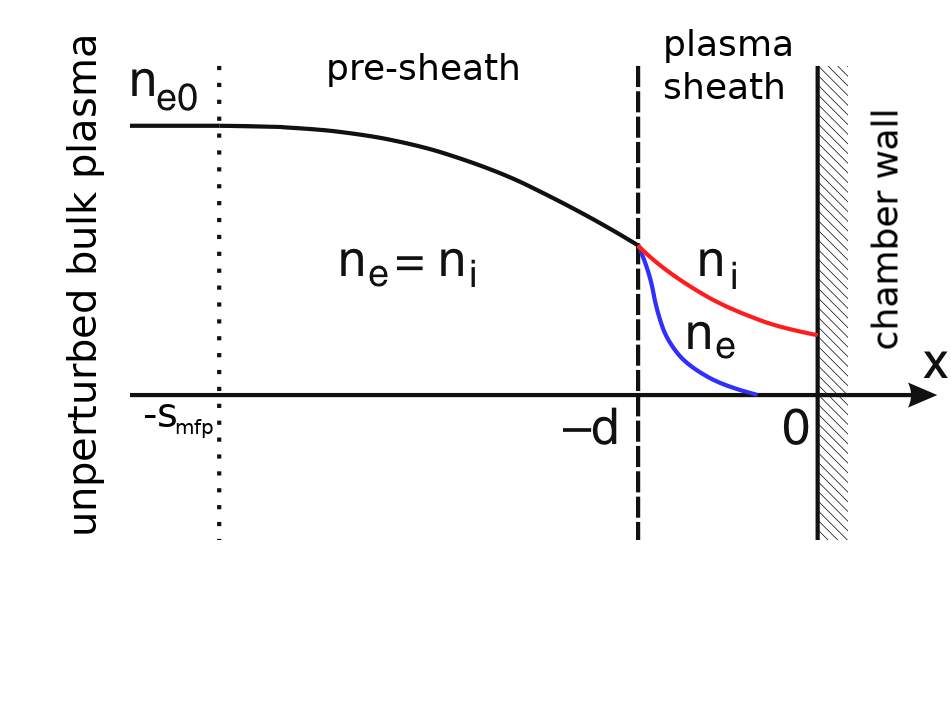
\includegraphics[width=0.6\textwidth]{figures/sheath_piel.png}%
				\caption{%
				One dimensional density profiles as a function of the distance to a floating wall. Note the exponential decrease of the electron density $n\ix{e}$ from the sheath border towards the presumably negatively charged wall. Densities allready reach approximately $0,66n\ix{e,0}$ inside the pre-sheath.~\cite{Piel10}}\label{fig:sheath_piel}
			\end{figure}
%
			For an instability, the force on the test body must increase with the distance from the equilibrium, hence the~\autoref{equ:inequality} is used to calculate the exact velocity at which an ion is entering the sheath. This results in the first \emph{Bohm criteria}.
%
			\begin{align}
				0>\left.\frac{\diff^{2}\Psi}{\diff\Phi^{2}}\right|_{\Phi=0}%
				\overset{\text{\autoref{equ:pseudo}}}{\overset{\mid}{=}}%
						\left.\frac{\diff}{\diff\Phi}\left(\frac{n\ix{e}\left(x\right)-n\ix{i}%
						\left(x\right)}{\varepsilon\ix{0}}\right)\right|_{\Phi=0}&%
						\frac{en\ix{e}\left(-d\right)}{\varepsilon\ix{0}}\left(\frac{e}%
						{k\ix{b}T\ix{e}}-\frac{e}{m\ix{i}v\ix{i,0}^{2}}\right)%
				\label{equ:condition}\\[10pt]%
				\Rightarrow\quad%
				v\ix{i,0}\ge v\ix{i,B}=\sqrt{\frac{k\ix{B}T\ix{e}}{m\ix{i}}}&%
				\label{equ:inequality}
			\end{align}
%	
			Analoguos you can define the so called \emph{Mach number} $M=v\ix{i,0}/v\ix{i,B}$, where $v\ix{i,B}$ denotes the \emph{Bohm velocity}.\\
			Now, to understand why the sheath does not extend further than a fixed distance $d$ from the discharge boundary, the particle movement has to be investigated on a smaller scale. As seen above, there is an electric field in the \emph{pre-sheath} that accelerates the ions to $v\ix{i,B}$. In addition, quasi-neutrality is still satisfied here:
%
			\begin{align}
				n\ix{i}\left(x\right)=n\ix{i,0}\exp\left(\frac{e\Phi\left(x\right)}{k\ix{B}T\ix{e}}\right)%
				=n\ix{e}\left(x\right)\,\,.%
				\label{equ:quasineutral}
			\end{align}
%
			Still, $\Phi{\left(x\right)}$ is the potential inside the pre-sheath from~\autoref{sec:sheathphysics} and $n\ix{i,0}$ the unperturbed density from the plasma \emph{bulk}. A greater part of the ion transport process in this area is governed by collisions with neutral gas particles, hence the velocity distribution function with the collision frequency $\nu\ix{n,i}$ has to be rewritten:
%
			\begin{align}
				\frac{\diff v\ix{i}}{\diff x}=\frac{\nu\ix{n,i}v\ix{i}^{2}}{v\ix{B}^{2}-v\ix{i}^{2}}\quad.%
				\label{equ:distribution}
			\end{align}
%
			From the singularity in~\autoref{equ:distribution} at $v\ix{i}=v\ix{B}$ and the knowledge of $\Phi(x)$ at the wall, one can calculate the sheath thickness $d$. Furthermore, ions with velocities smaller than the Bohm velocity are being accelerated inside the pre sheath. According to~\autoref{equ:inequality} velocities greater than $v\ix{B}$ are not allowed here. This is, together with~\autoref{equ:distribution} the reason why the ion velocity is exactly $v\ix{B}$ at the boundary of the plasma sheath and thus a positive space-charge ensues.
%
			\begin{align}
				M\ge1%
				\Leftrightarrow%
				v\ix{i}(-d)\ge v\ix{B}%
				\label{equ:bohmcriteria2}
			\end{align}
%
			Conclusively, at the sheath boundary~\autoref{equ:bohmcriteria2} is satisfied.\\
			At $x=-d$, both negative and positive charge density decreased to $n\ix{i}=n\ix{e}\approx0,66n\ix{e,0}$ (see~\autoref{fig:sheath_piel}), where the potential is approximately $-k\ix{B}T\ix{e}/2e$ because of the currents onto the wall.\\
			In summarization, the plasma does not `see' its sheath, because the ion dynamic discussed before is spatially restricted. The sheath only develops where there is electron depletion or an externally applied, negative potential.
%
			\subsection{Self Bias Voltage}\label{sec:selfbias}
%
				An important step towards the electric characterization of such ccrf discharges is the development of a replacement circuit, see~\autoref{fig:replacementcurrent}. Thus, one can define a specific impedance for a rf discharge of excitation frequency $\omega$. The value of $\varepsilon\ix{p}$ resembles the permeability of the working gas between the driven and/or grounded electrode~\cite{Piel10}. In addition, this volume has the capacity $C\ix{p}$ --- the capacity of a cubicle with a cross section $A$, thickness $b$ and electron-neutral collision frequency $\nu\ix{e,n}$ calculates like~\autoref{equ:capacityandepsilon}.
%
				\begin{align}
					\varepsilon\ix{p}=&1-\frac{\omega\ix{p,e}^2}{\omega\left(\omega-\imag\nu\ix{e,n}\right)}\,,%
						\quad\quad%
						C\ix{p}=\varepsilon\ix{p}C\ix{0}=%
						\varepsilon\ix{p}\varepsilon\ix{0}\frac{A}{b}%
						\label{equ:capacityandepsilon}\\[0.2cm]
					&Z\ix{p}={\left(\imag\omega C\ix{p}+ \frac{1}{\frac{1}{\omega\ix{p,e}^2C\ix{0}}%
							{\left(\nu\ix{e,n}+\imag\omega\right)}}\right)}^{-1}%
					\label{equ:bulkimpedanz}
				\end{align}
%		
				\begin{figure}[!b]
					\centering
					\begin{subfigure}[b]{0.49\textwidth}
						\centering%
						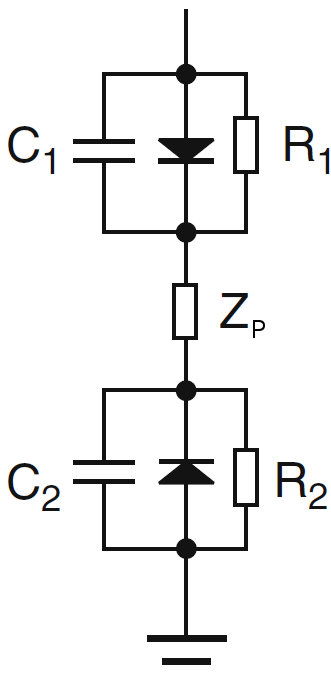
\includegraphics[width=0.4\textwidth]{figures/circuit_selfbias_piel.png}
						\caption{Replacement Circuit}\label{fig:replacementcurrent}
					\end{subfigure}
					\begin{subfigure}[b]{0.49\textwidth}
						\centering%
						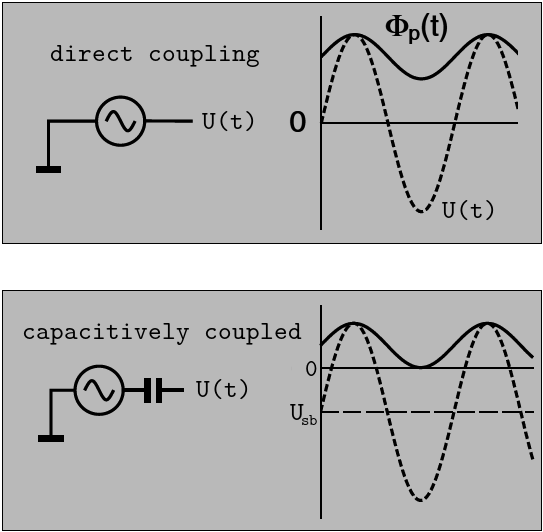
\includegraphics[width=0.8\textwidth]{figures/selfbiasvoltage.png}
						\caption{Voltage and Potential}\label{fig:circuitselfbias_2}
					\end{subfigure}
						\caption{%
							Figure for an asymmetrically driven ccrf discharge.~\cite{Piel10}\\%
						(A): $Z\ix{p}$ denotes the impedance of the plasma bulk. A diode represents the directed electron current from the sheath into the discharge volume. $R\ix{j}$ and $C\ix{j}$ are the electrical properties of the positive space-charge area.\\%
					(B): Schematic of potential and voltage of a direct capacitively coupled rf discharge.}%
				\end{figure}
%
				The~\autoref{equ:bulkimpedanz} represents the full electrical impedance, consisting of the inverse sum of real and imaginary resistance, as well as the capacity of the neutral gas volume. Here, $\imag\omega/(\omega\ix{p,e}^{2}C\ix{0})$ characterizes the electrons inertia in regard to an external excitation $\omega$. The real part $\nu\ix{e,n}/(\omega\ix{p,e}^{2}C\ix{0})$ denotes the resistance by neutral particle collisions.\\
				For high excitation frequencies, e.g.\@ $\unit[13,56]{MHz}$ the bulk impedance can be neglected (see~\autoref{equ:bulkimpedanz},~\cite{Kay85}). Both sheath capacities of anode and cathode take the dominant part. Therefore, the discharge potential and voltage can be written as:
%
				\begin{align}
					U\left(t\right)=U\ix{sb}+U\ix{rf}\sin\left(\omega t\right)\,,%
						\quad\quad%
						\Phi\ix{p}\left(t\right)=\overline{\Phi\ix{p}}+%
						\Phi\ix{rf}\sin\left(\omega t\right)%
					\label{equ:selfbias_1}
				\end{align}
%
				Both electrodes sheath collapses completely during a full cycle of $U\ix{rf}(t)$, which is why charges can impinge onto the surface and force the plasma potential $\Phi\ix{P}$ to equal out locally with the walls. A short circuit between plasma and sheath occurs when $\Phi\ix{P}$ becomes negative with regard to the excitation. The~\autoref{equ:selfbias_unequal} and~\autoref{fig:circuitselfbias_2} express this circumstance.
%
				\begin{align}
					\Phi\ix{p}\max=\overline{\Phi\ix{p}}+\Phi\ix{rf}\geq U\ix{sb}+U\ix{rf}\,,%
						\quad\quad %
						\Phi\ix{p}\min=\overline{\Phi\ix{p}}-\Phi\ix{rf}\geq0%
						\,\,.%
					\label{equ:selfbias_unequal}
				\end{align}
%     
				If there is no special coupling between electrode and electrical driver, the equality in~\autoref{equ:selfbias_unequal} is true. However, if a capacitive coupling is used, there can't be any net current between excitation and electrode. The capacitance can not be inverted over the course of one rf cycle. The electron currents are then equal on both electrodes, therefore shifting the minimum plasma potential to ground and the maximum to the excitation.\\
				Finally, the dc \emph{self bias} part $U\ix{sb}$ and the mean plasma potential $\overline{\Phi\ix{p}}$ are
%
				\begin{align}
					\overline{\Phi\ix{p}}=\frac{1}{2}\left(U\ix{sb}+U\ix{rf}\right)\,,%
						\quad\quad%
						U\ix{sb}=\frac{C\ix{1}-C\ix{2}}{C\ix{1}+C\ix{2}}U\ix{rf}%
						\,\,.%
					\label{eq:selfbiaszwei} 
				\end{align}
%     
				If the excitation frequency $\omega$ is small compared to other time scales, e.g\@ electron and ion plasma frequencies, the electron current from the sheath $j\ix{L}$ becomes bigger than the displacement current $j\ix{dc}$. Hence the electron current onto the driven electrode decreases by a maxwellian factor --- this is a function of the thereon apllied voltage --- compared to the corresponding ion current.\\
				Conclusively, the electrodes sheath impedance is bigger than those of the floating walls. Together with~\autoref{equ:selfbias_1} and~\autoref{equ:inequality} the plasma potential $\Phi\ix{p}$ approximately vanishes, requiring only the currents onto the driven electrode to equal out. For small values of $\omega$~\autoref{equ:selfbias_3} yields the \emph{self bias voltage}~\cite{Piel10}. Here, $\mathbf{J}\ix{0}$ denotes the zeroth order \emph{Bessel function}.
%      
				\begin{align}
					U\ix{sb}=\frac{k\ix{B}T\ix{e}}{e}\ln%
						\left[\mathbf{J}\ix{0}\left(\frac{eU\ix{rf}}{k\ix{B}T\ix{e}}\right)\right]%
					\label{equ:selfbias_3}
				\end{align}
%     
% TODO: fig:imagandreal :TODO
%
				In (insert fig:imagandreal here) the voltage's real and imaginary part are shown for an exemplary ccrf discharge. One can examine there that the self bias never disappears for excitations $U\ix{rf}\neq0$, hence becoming an important part for capacitively coupled plasma.
%
			\subsection{Dielectric Displacement Current}\label{sec:displacementcurrent}
%
				\begin{wrapfigure}{r}{0.47\textwidth}
					\centering%
					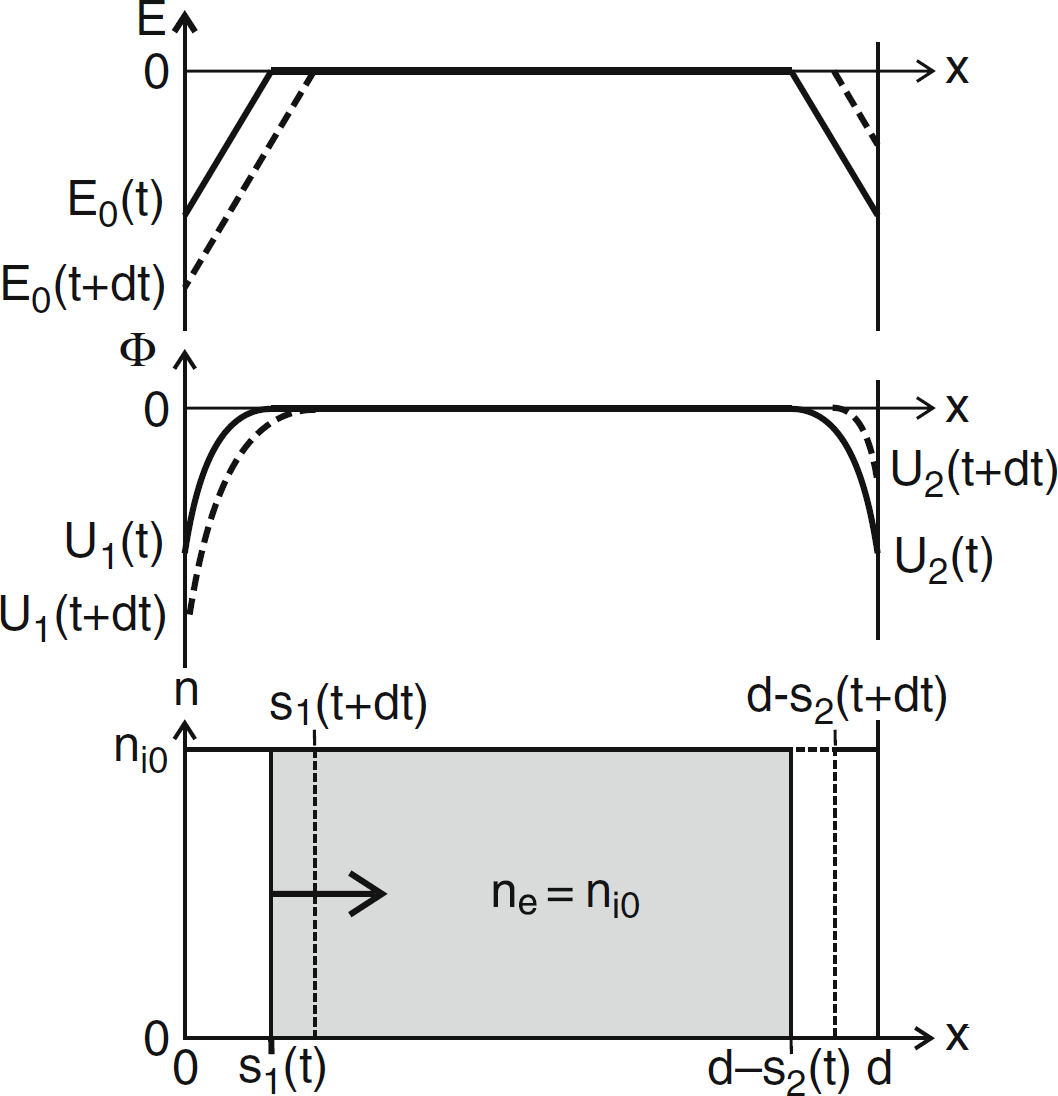
\includegraphics[width=0.45\textwidth]{figures/displacement_current_piel.png}%
					\caption{%
					One dimensional density, potential and electric field for an asymmetric, harmonically driven discharge. Note the moving sheaths border.~\cite{Piel10}}\label{fig:displacementcurrent}
				\end{wrapfigure}
%
				Due to their higher mobility and plasma frequency $\omega\ix{p,e}$, the electron distribution can follow an external excitation with a similarly high frequency much better than the heavier ions species. Because of that, one will assume those as nearly stationary, e.g.\@ $\omega\ix{p,i}\ll\omega\ix{p,e},\,\omega\ix{rf}\,$. Investigating the circumstances and consequences of this relation yields the displacement current $j\ix{d}$. \\
				Lets suppose there is an area of thickness $d$ in front of a negatively charged wall, where the electron ensity is negligible and the corresponding ion property constant at $n\ix{0,i}$. Thus an electric field of
%   	 
				\begin{align}
					E\ix{0}=-en\ix{0,i}d/\varepsilon\ix{0}
				\end{align}
%
				establishes. If the wall potential now decreases due to electron bombardment or external manipulation, the sheaths border moves further inside into the discharges volume with the velocity $u\ix{s}=\diff s\ix{1}/\diff t$. Thus, the sheath expansion and hence charge movement creates an additional \emph{displacement current} $j\ix{d}$, which is compensated with $j\ix{d,e}$ the electron current from this border displacement. Hence charge conservation and continuity is satisfied~\cite{Godyak90a}.
%
				\begin{align}
					j\ix{d}=-en\ix{0,i}u\ix{s}=-j\ix{d,e}
				\end{align}
%
				Electrons that are pushed out of this positive space-charge area then contribute to the plasma bulk density, and conclusively, to the quasi neutrality $n\ix{e}=n\ix{0,i}\,$. But in case of a harmonically driven discharge, the sheath in front of the opposing electrode is shrinking with $\diff s\ix{1}=-\diff s\ix{2}\,$. Hence, the bulks spatial expansion and position are oscillating sinusoidal, or: the sheaths thickness oscillates harmonically around a mean value, e.g\@ $s\ix{0}$. The associated voltage drop across the discharge~\cite{Piel10} between the sheath potentials $U\ix{1/2}$ would be
%
				\begin{align}
					\Delta U=U\ix{1}-U\ix{2}=-\frac{2en\ix{i,0}s\ix{0}}{\varepsilon\ix{0}}\exp{\left(\imag\omega t\right)}
				\end{align}
	%
		\subsection{Heating Mechanisms}\label{sec:heating}
%
		\paragraph{Ohmic Heating}
		In a spatially uniform electric field thas oscillates perpendicular to the electrodes harmonically, like it is the case in the bulk of a previously concerned ccrf discharge, electrons periodically gain and loose energy in the absence of collisions without any net energy gain~\cite{Schulze09}. This is due to the simmetrical de-/acceleration in the sheaths an main plasma volume over one rf cycle. Lets assume the electric field have no or a negligiable component parallel to the electrodes. Hence the mean absorbed power by the electrons in an oscillating electric field is
%
		\begin{align}
			\overline{P}\ix{ohm}=\omega\ix{rf}\int_{0}^{T\ix{rf}}\,j\ix{tot}(t)\cdot E(t)\diff t%
			\label{equ:meanpowerheat}\\[0.0cm]%
			m\ix{e}\frac{\diff v\ix{e}}{\diff t}=-eE(t)-m\ix{e}\nu\ix{n,e}v\ix{e}%
			\label{equ:heatingmotion}
		\end{align}
%
		The total charge current density $j\ix{tot}$ is the sum of displacement current from~\autoref{sec:displacementcurrent} and conduction current $en\ix{e,0}v\ix{e}\,$. Solving~\autoref{equ:heatingmotion} for the velocity, one yields and imagniary and real part due to the bulks impedance, like it was discussed earlier in~\autoref{sec:selfbias}. Substitution of this result~\cite{Schulze09} gives
%
		\begin{align}
			\overline{P}\ix{ohm}=\frac{|E\ix{0}|^{2}\Re(\sigma\ix{p})}{2}=%
			\frac{|j\ix{0}|^{2}}{2\Re(\sigma\ix{p})}\,,%
			\quad\quad%
			\sigma\ix{p}=\frac{n\ix{e}e^{2}}{m\ix{e}(\nu\ix{n,e}+\imag\omega\ix{p})}%
			\label{equ:ohmicheating}
		\end{align}
%
		This is, again, the total mean power dissipated into the electron species through accelration in a harmonically oscillating electric field and neutral gas friction. The property $\sigma\ix{p}$ is the plasma conductivity, hence yielding $j\ix{0}=\sigma\ix{p}E$. This shows that power from an spatially uniform, harmonically oscillating electric field can only be transferred via collisions. Elastic electron-neutrals collision transferred into a direction perpendicular to the field and is, hence, not lost during the reversal of $E(t)$. Therefore the electron species gains energy during the field oscillation. This mechanism is called \emph{ohmic heating} and takes place mainly in the plasma bulk.
%
		\paragraph{Stochastic Heating}
		Low-pressure, capacitively coupled rf plasma can primarily be stabilzed by collisionless heating in the sinusoidally  modulated discharge sheaths, like it was proposed earlier in~\autoref{sec:langmuirlaw} and the following. Most theoretical models assume a `hard wall' approximation (HWA), where the electrons are cosidered to collide elastically with the oscillating sheath edge. Heating power is then averaged by reverse and forward energy fluxes into and out of the sheath respectively. This gives an easy access to heating mechanisms of the proposed discharges.\\
		The heating mechanism in such low pressure plasma is of particular importance, because collisions are rare and sheath processes are key to the sustainabilty of the discharge (see e.g\@~\autoref{sec:bohmcriteria}). The afore-mentioned HWA uses the '\emph{fermi acceleration}' argument, which implies that the particles are heated or cooled due to the sheaths sinusoidal oscillation and a corresponding de-/accelration. This process, though relying on enough randomization in phase-space inside the bulk, sufficiently creates a net heating of the plasma~\cite{Gozadinos01b,Goedde88}. This is referred to as \emph{stochastic heating}.\\
		Here one will consider the sheaths electric field as constant, $E=U\ix{sb}/s\ix{0}$, the bulks expansion to be $l$  and the sheaths thickness $d$ being modulated cosinusoidal. The equation of motion for an electron in the sheath is taken from above, canceling out the part of ohmic neutral gas heating.
%
		\begin{align}
			d(t)\approx s\ix{0}\left(1+\frac{U\ix{rf}}{U\ix{sb}}\cos\left(\omega t\right)\right)%
			\label{equ:sheaththickness}
		\end{align}
%
		The~\autoref{equ:heatingmotion} is introduced as dimensionless with the corresponding parameters: $\alpha=m\ix{e}\omega^{2}s\ix{0}^{2}/(eU\ix{sb})$, $\beta=U\ix{rf}/U\ix{sb}$ and $\epsilon=s\ix{0}/l\,$. Integrating yields the velocity $\mu(\tau)$ of an electron as it moves through the sheath. The transit time $\tau$ is considered for one pass through the sheath of the particle. It can be used to calculate the change in velocity experienced by the electron on each bounce between this oscillating and a fixed wall --- this would be the lowest order \emph{fermi acceleration}. Assuming there are two distinct points in motion, where the particle enters (index $n$) and re-enters (index $n+1$) the sheath, this gives, using $\varphi\ix{n}$ the phase of the sheath, for the transit time and velocity~\cite{Goedde88}
%
		\begin{align}
			\tau\ix{n}\approx\frac{2\alpha(\mu\ix{n}-\beta%
				\cos\varphi\ix{n})}{1+\alpha\beta\cos\varphi\ix{n}}\,,%
			\quad\quad%
			\mu\ix{n+1}=-\mu+\frac{2(\mu\ix{n}-\beta\sin\varphi\ix{n})}{1+\alpha\beta\cos\varphi\ix{n}}%
			\label{equ:transitandvelocityheating}
		\end{align}
%
		In \emph{hamiltonian mappings}, those two variables are not canonically conjugate, hence insufficient for checking conservational properties. One has to keep that in mind when evaluating the HWA approximation. The change in velocity in one pass through the sheath becomes the impulse approximation of the \emph{Fermi acceleration}. Here, written again with common variables.
%
		\begin{figure}[b!]
			\centering
			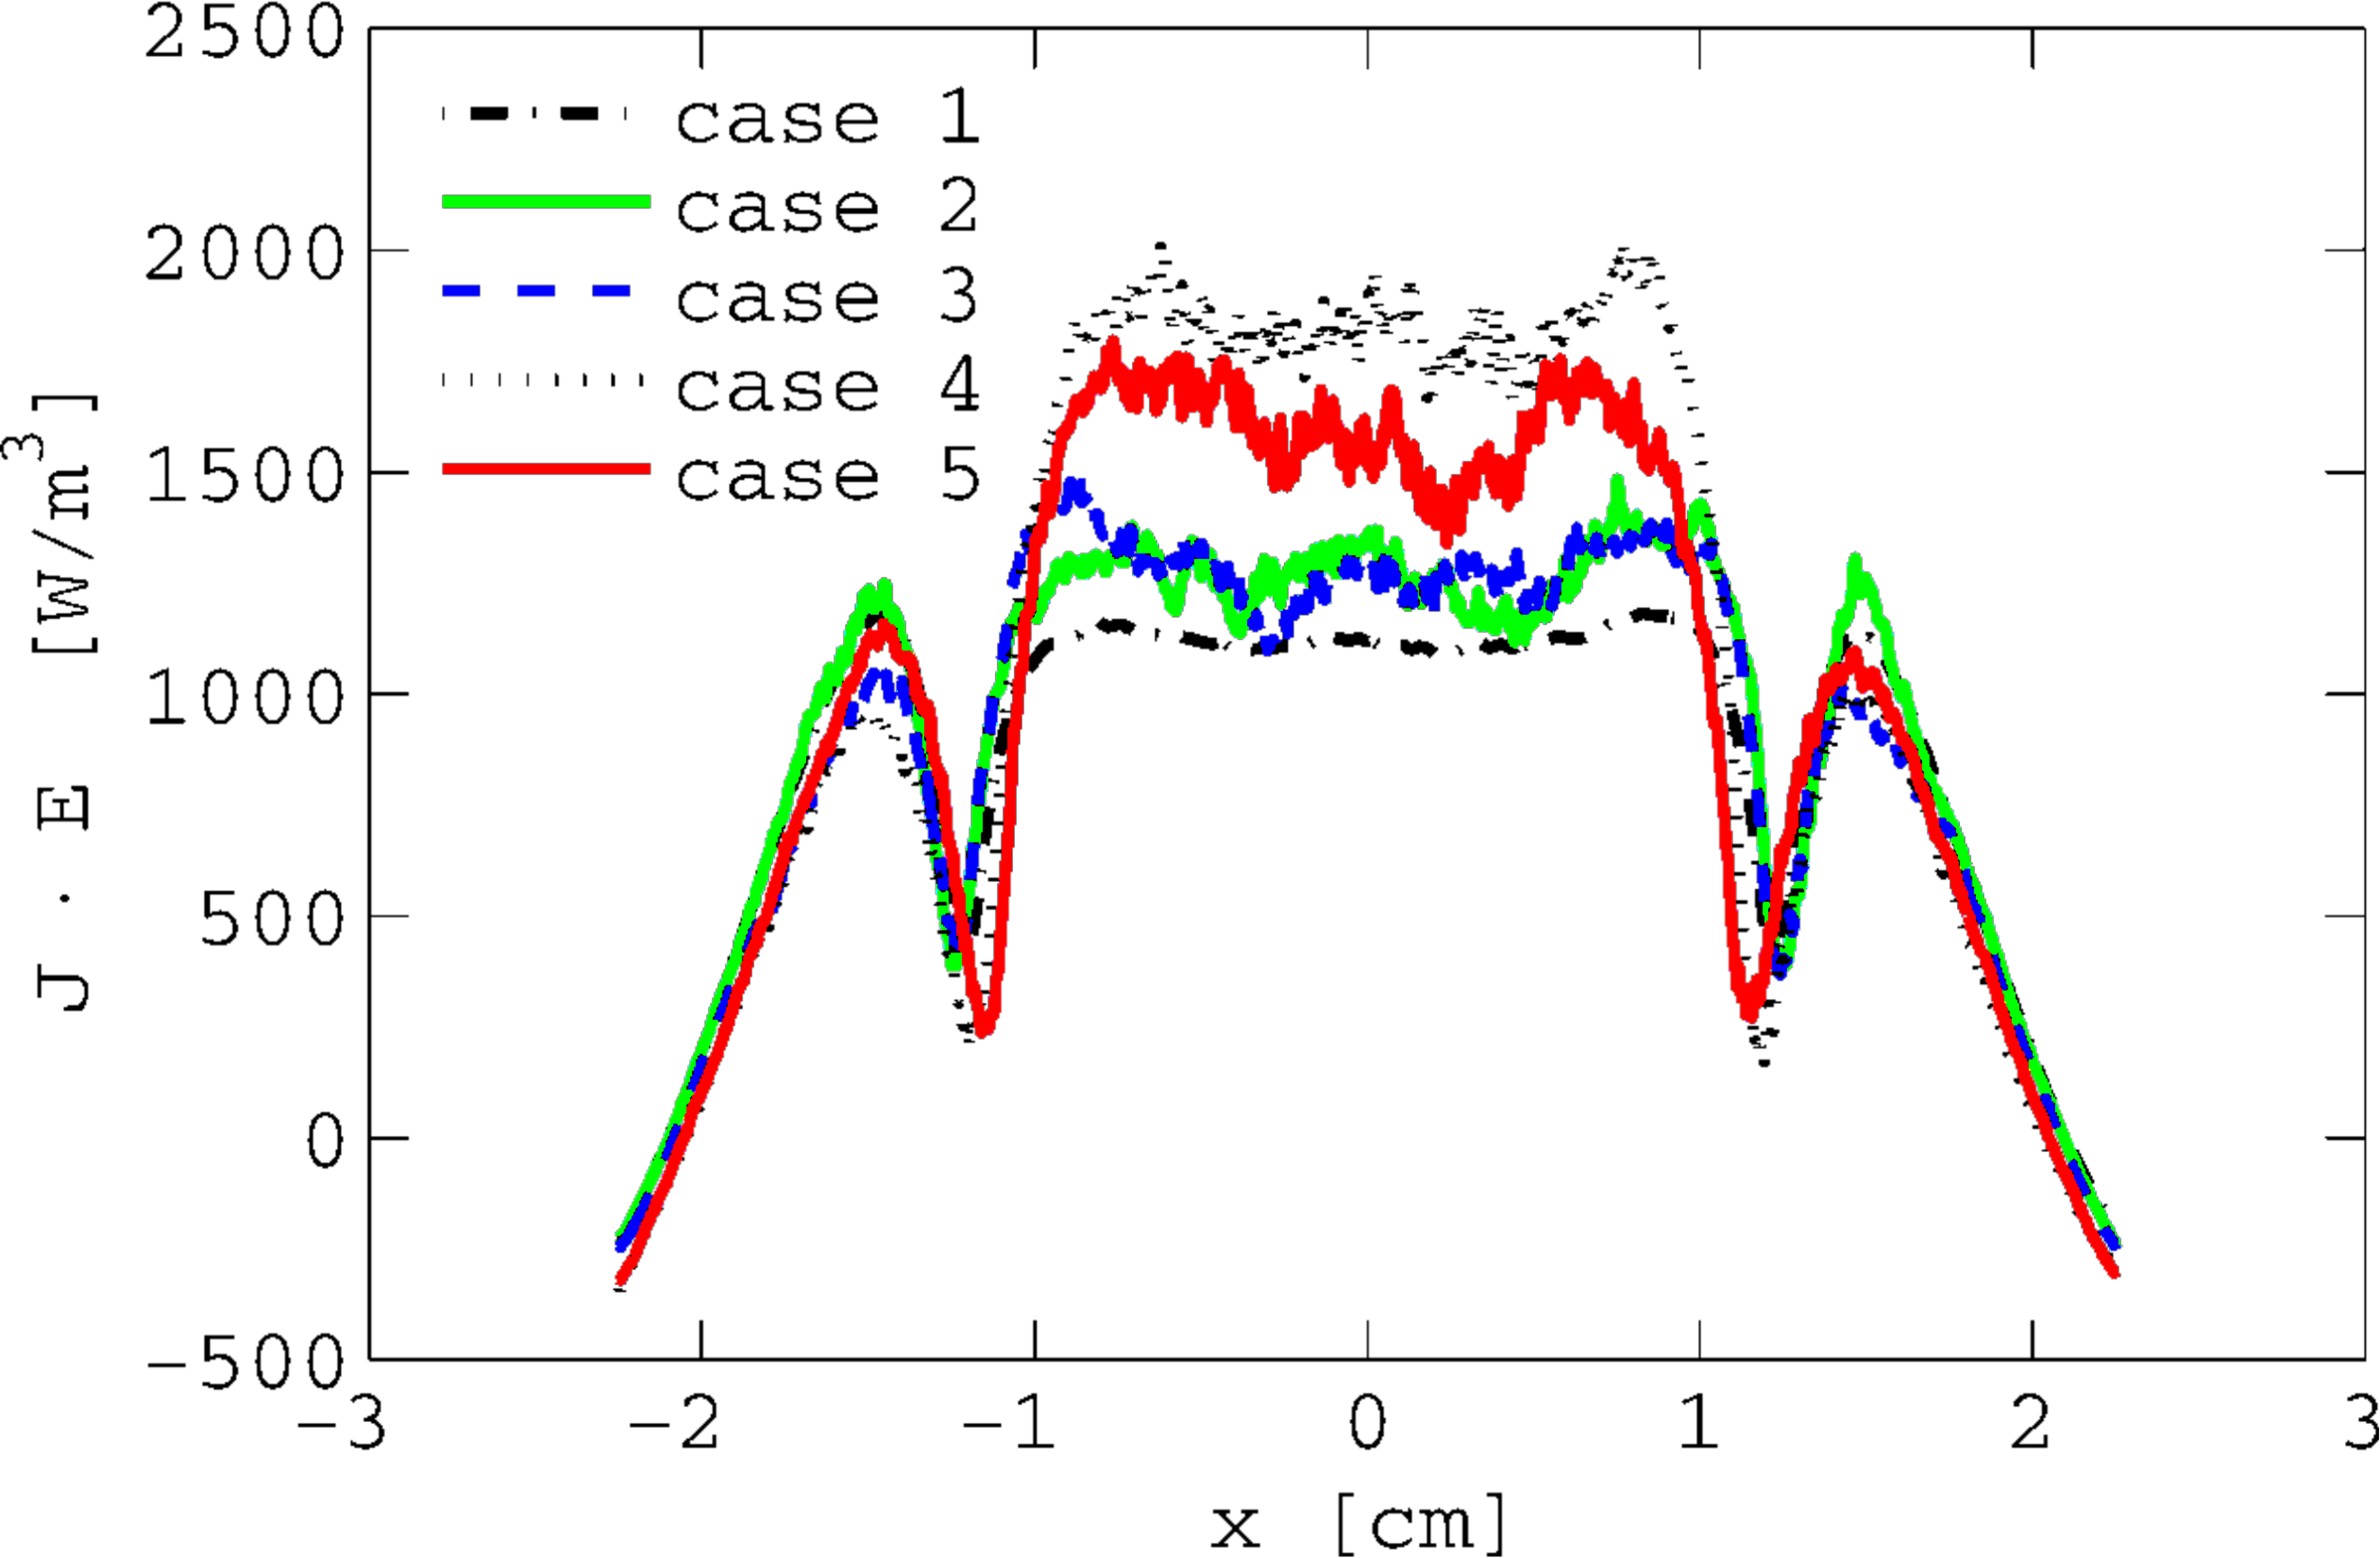
\includegraphics[width=0.7\textwidth]{figures/heatingcomparison.pdf}
			\caption{%
			Electron heating rate for a ccrf discharge of parallel plates at $\unit[6,7]{Pa}$ with an electrode gap of $\unit[4,5]{cm}$ at $\unit[222]{V}$. Other corresponding plasma parameters are noted in~\autoref{tab:comparisonheating}.~\cite{Gudmundsson13}}\label{fig:heatingcomparison}
		\end{figure}
%		
		\begin{figure}[t!]
			\centering
  		\begin{longtable}{lccccr}
				\toprule%
					Case & $\Phi\ix{0}$ & $n\ix{e,0}$/$\unit{m^{-3}}$ %
					& $n\ix{i-,0}$/$\unit{m^{-3}}$ & $n\ix{i+,0}$/$\unit{m^{-3}}$ %
					&	$T\ix{e,0}$/$\unit{eV}$ \\%
		    \toprule\midrule\endhead%
				1 & 101,30 & $2,43\cdot\tenpo{14}$ & $1,17\cdot\tenpo{16}$ %
				& $1,20\cdot\tenpo{16}$ & 2,83 \\ \midrule%
				2 & 101,25 & $2,29\cdot\tenpo{14}$ & $1,21\cdot\tenpo{16}$ %
				& $1,23\cdot\tenpo{16}$ & 2,98 \\ \midrule%
				3 & 101,75 & $2,18\cdot\tenpo{14}$ & $1,19\cdot\tenpo{16}$ %
				& $1,20\cdot\tenpo{16}$ & 2,98 \\ \midrule%
				4 & 103,11 & $1,55\cdot\tenpo{14}$ & $1,75\cdot\tenpo{16}$ %
				& $1,78\cdot\tenpo{16}$ & 3,59 \\ \midrule%
				5 & 102,55 & $1,65\cdot\tenpo{14}$ & $1,70\cdot\tenpo{16}$ %
				& $1,71\cdot\tenpo{16}$ & 3,43 \\ \midrule%
    	\bottomrule%
			\caption{%
				Selected plasma parameters for the used cases in~\autoref{fig:heatingcomparison} at the center of the discharge.~\cite{Gudmundsson13}}\label{tab:comparisonheating}
			\end{longtable}
		\end{figure}
%
		\begin{align}
			\Delta v=v\ix{n+1}-v\ix{n}=-2\,\omega\,%
			s\ix{0}\frac{U\ix{rf}}{U\ix{sb}}\,\sin\varphi\ix{n}%
			\label{equ:deltavheating}
		\end{align}
%	
		A question to answer is what parameter defines the degree of randomization required for an ample stochastical heating in the plasma sheath. Therefore, $K$ is defined as a function of phase-space chaos by eletron energy. Additionally, a simple condition for stochastical motion is derived at the same time.
%
		\begin{align}
			K=\alpha\,\beta\,\frac{U\ix{sb}}{\epsilon E}\,,%
			\quad\quad%
			E\,<\,m\ix{e}\,\omega^{2}s\ix{0}\,l\,\frac{U\ix{rf}}{U\ix{sb}}%
			\label{equ:randomization}
		\end{align}
%
		As is well known~\cite{Goedde88}, chaotic motion occurs in this mapping for $K>1$. It decreases with increasing energy, so the system is less stochastic at higher energies. This is due to the shrinking phase shift across the discharge volume with higher energies. Hence phase corellations between successive collisions in and with the plasma sheath reduce stochasticity.\\
		Last, but not least, one calculates the instantaneous power dissipated into the plasma due to this heating mechanism. Here, using the sheath speed from above $u\ix{s}$, the electron drift velocity $u\ix{e}$ and the maxwellian electron velocity distribution funtion $f\ix{v}(v\ix{e},t)$, Lieberman~\cite{Lieberman88} finds
%
		\begin{align}
			P\ix{stoc}(t)=-2m\ix{e}\int_{u\ix{s}}^{\inf}\,u\ix{s}%
			{\left(v\ix{e}-u\ix{s}\right)}^{2}\,f\ix{v}(v\ix{e},t)\diff v=%
			2\,n\ix{e,0}u\ix{e}k\ix{B}T\ix{e}\sin(\omega t)%
			\label{equ:powerdepositheat}
		\end{align}
%
		Clearly, this results yields not net heating if averaged over one rf cycle. That is, if the current used would be conserved in a manner the HWA is predicting it, or the electron drift velocity does not satisfy the maxwellian distribution function. Hence, there have to be deviations from the proposed theory of stochastical heating. This would be e.g.\@ ab initio information about the EEDF, unconsidered transit time effects of the sheath electric field and neglected particle losses and current conservation.\\
		Therefore more theoretical approaches on the heating in low-pressure, low-temperature rf plasma. For example, Surendra et al~\cite{Surendra93} put forth the idea that the compression and decompression of the electron density volume between opposing plasma sheaths generates heat inside the bulk is responsible for the observed heating.\\
		The electron heating profile is shown in~\autoref{fig:heatingcomparison}. The electron heating peaks near the sheath edges are due to the stochastic heating while the main plateau in the bulk is a result of the dominantly strong ohmic heating with slow electrons and neutral gas friction.

	%
	\section{Oxygen Plasma Chemistry}\label{sec:negionphysics}
%
		In comparison to most inert working gases in ccrf discharges, oxygen has an overwhelming number of reaction sets for collisions of elastic, inelastic and reactive character. Additionally, the negative ion species has to be taken into account when discussing collisional processes. For example, an in-depth benchmarking of both simulated and experimentally measured cross section data is given by Gudmundsson et al.\@ in~\cite{Gudmundsson13}. There, 33 collisions and reactions have been revisited, already reducing the investigation to the most important processes in ccrf plasma. In this thesis the selection of possible reactions will be based on~\cite{Bronold07b} and slightly modified. The final collection of cross sections can be found in~\autoref{tab:cross_sections} and observed in~\autoref{fig:cross_sections_mine}. Those data are semi-empirical, meaning part of them are based on measurements in finite energy ranges and low-/high-energy asymptotic models. Cross sections for very high energies are not important, as the collision probability usually decays very fast here.\\
		As already seen in~\autoref{sec:heating}, collisions strongly influence the particle distribution functions and density profiles. Furthermore, a good understanding of the plasma chemistry is key to, e.g.\@ applications in surface physics supported by gas discharges. Of high importance for plasma-assisted material processes is the generation of negative ions. Hence the ratio $\alpha=n\ix{i,-}/n\ix{e}$ is important to characterize the electronegative plasma, like a ccrf oxygen discharge by $\alpha>1$.\\
		I will highlight the most important collisions and reactions in the following section. 
%
		\begin{longtable}{lll}
			\toprule%
				\bfseries Nr. & \bfseries Reaction & \bfseries Type \\%
			\toprule\midrule\endhead%
						& \bfseries Elastic scattering 							& \bfseries Energy loss 	\\% 
						$(1)$  & $e^{-}+O\ix{2}			 	\rightarrow	O\ix{2}+e^{-}$ &						\\%
						$(2)$  & $O^{-}+O\ix{2}			 	\rightarrow	O\ix{2}+O^{-}$ & 						\\%
						$(3)$  & $O\ix{2}^{-}+O\ix{2} \rightarrow	O\ix{2}+O\ix{2}^{-}$ & 			\\ \midrule%
						& \bfseries Electron energy loss scattering & \bfseries Energy loss 	\\%
						$(4)$  & $e^{-}+O\ix{2}			 	\rightarrow	O\ix{2}^{\nu}+e^{-}$ & %
										Vibrational excitation	($\nu=1,\dots,4$)											\\%
						$(5)$  & $e^{-}+O\ix{2}			 	\rightarrow	O\ix{2}(Ryd)+e^{-}$ & %
										Rydberg excitation																						\\%
						$(6)$  & $e^{-}+O\ix{2}			 	\rightarrow	O(1D)+O(3P)+e^{-}$ & %
										Dissociative excitation at $\unit[8,6]{eV}$										\\%
						$(7)$  & $e^{-}+O\ix{2}		 	 	\rightarrow	O\ix{2}%
																					 (a^{1}\Delta\ix{g},b^{1}\Sigma\ix{g})$ & %
										Meta-stable excitaion																					\\ \midrule%
						& \bfseries Electron and ion reactions & \bfseries Creation and loss 	\\%
						$(8)$  & $e^{-}+O\ix{2}^{+}	 	\rightarrow	2\,O$ & %
										Dissociative recombination 																		\\%
						$(9)$  & $O^{-}+O\ix{2}^{+}	 	\rightarrow	O\ix{2}+O$ & %
										Neutralization						 																		\\%
						$(10)$ & $e^{-}+O\ix{2}	 		 	\rightarrow	O+O^{-}$ & %
										Dissociative attachment		 																		\\%
						$(11)$ & $O^{-}+O\ix{2}			 	\rightarrow	O+O\ix{2}+e$ & %
										Direct detachment 																						\\%
						$(12)$ & $e^{-}+O\ix{2}		 		\rightarrow	2e^{-}+O\ix{2}^{+}$ & %
										Impact ionization 																						\\%
						$(13)$ & $e^{-}+O^{-}			 		\rightarrow	O+2e^{-}$ & %
										Impact detachment																							\\%
			\midrule\bottomrule%
			\caption{%
				Most important colilision and reactions in ccrf plasma with the largest cross sections. %
				Empirical and simulated data, which have been included in this simulation are shown in~\autoref{fig:cross_sections}.}\label{tab:cross_sections}	
		\end{longtable}	
%		
		\subsection{Collisions and Reactions}\label{sec:negiondynamics}
%	
			The elastic collisions of $(1)--(3)$ conserve the particle numbers. Those are inter-species scattering processes, which will be assumed to have an isotropic inincident angle dependency~\cite{Bronold07b}. Intra-species elastic collisions were not very important at the selected parameter regions, though ion-ion scattering can strongly incluence the IEDF structure of the concerned densities are very high. However, for the electron species a binary \emph{coulomb scattering} process was used: the scattering angle $\chi$ is given by~\autoref{equ:coulomb_scatter} with $v\ix{rel}$ the relative velocity, $\ln\Gamma$ the Coulomb logarithm (see~\autoref{tabe:physicalquantities}) and $\tau\ix{c}$ the collision time.
%
			\begin{align}
				\langle\tan^{2}\frac{\chi}{2}\rangle=\frac{e^{4}n\ix{e}\ln\Gamma}%
					{8\pi\varepsilon\ix{0}m\ix{e}^{2}v\ix{rel}^{3}}\tau\ix{c}%
				\label{equ:coulomb_scatt}	
			\end{align}	
%
			The~\autoref{fig:cross_sections} shows the corresponding cross sections. In fact, only two are elastic processes, where as the collision of $O\ix{2}^{+}$ and the neutral molecule is a charge exchange reaction with momentum transfer. This kind of process:
%
			\begin{align}
				A^{-/+}+B\rightarrow A+B^{+/-}%
				\label{equ:charge_exchange}
			\end{align}
%
			is important for the consideration of surface effects. An ion with greater than thermal velocity coming from the wall will be cooled down by charge exchange collisions, which will transfer heat into the neutral reservior.\\

%			
			\begin{figure}[!b]
				\centering
				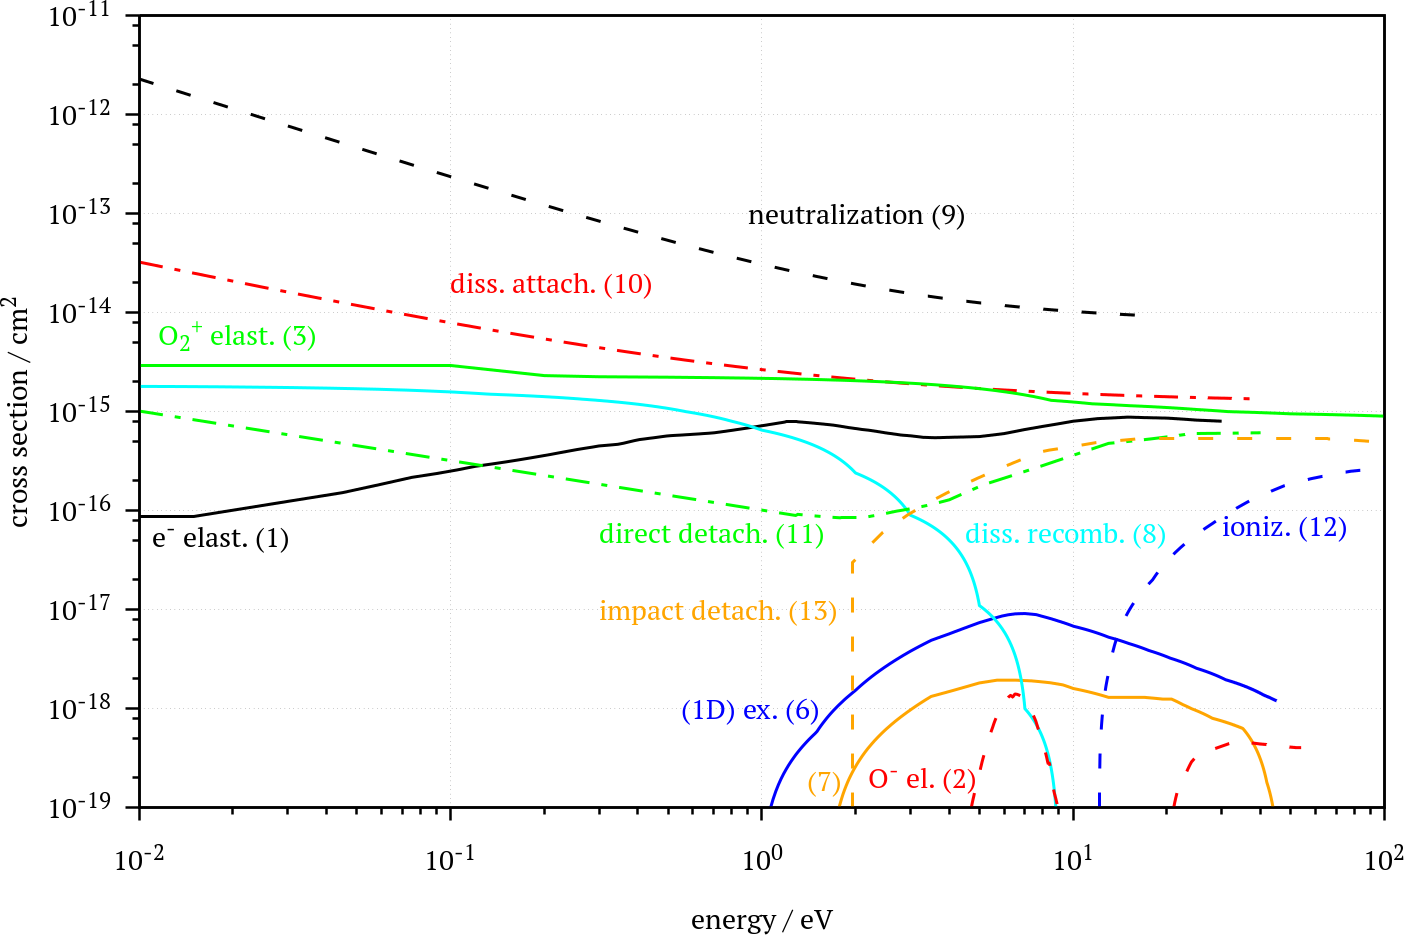
\includegraphics[width=1.0\textwidth]{figures/xsections.png}
				\caption{%
					Test.}%
				\label{fig:cross_sections}	
			\end{figure}	

%			
		\subsection{Anion Production}\label{sec:anionproduction}
%

	%
	\section{Particle-in-Cell Simulations with Monte Carlo-Colissions}\label{sec:picsimulationmcc}
%
		\subsection{Principles}\label{sec:picbasics}
%
		\subsection{2d3v PIC}\label{sec:pic_2d3v}
%
		\subsection{Monte Carlo-Collisions}\label{sec:montecarlo}
%

% RESULTS
	%
\chapter{Validation of Simulation by 1d comparison}\label{sec:chapter_onedcomparison}
%
	\section{Axial density profiles}\label{sec:onedprofiles}
%
	\section{Velocity and energy distributions}\label{sec:onedvelocities}
%
	\section{Transition to 2d simulation}\label{sec:onedtransition}
%

	%
\chapter{Simulation of capacitively coupled rf discharges}\label{sec:chapter_twodccrf}
%
	\section{Experimental setup}\label{sec:twod_setup}
%
		Giving the necessary background in~\autoref{sec:surfaceeffects} and providing the crucially important comparison of the previous~\autoref{sec:chapter_onedcomparison}, the afore-mentioned effects of highly energetic negative oxygen ions can now be further investigated.
%
		\subsection{Reference Discharge}\label{sec:reference_dis}
%
			\begin{figure}[b!]
				\centering
				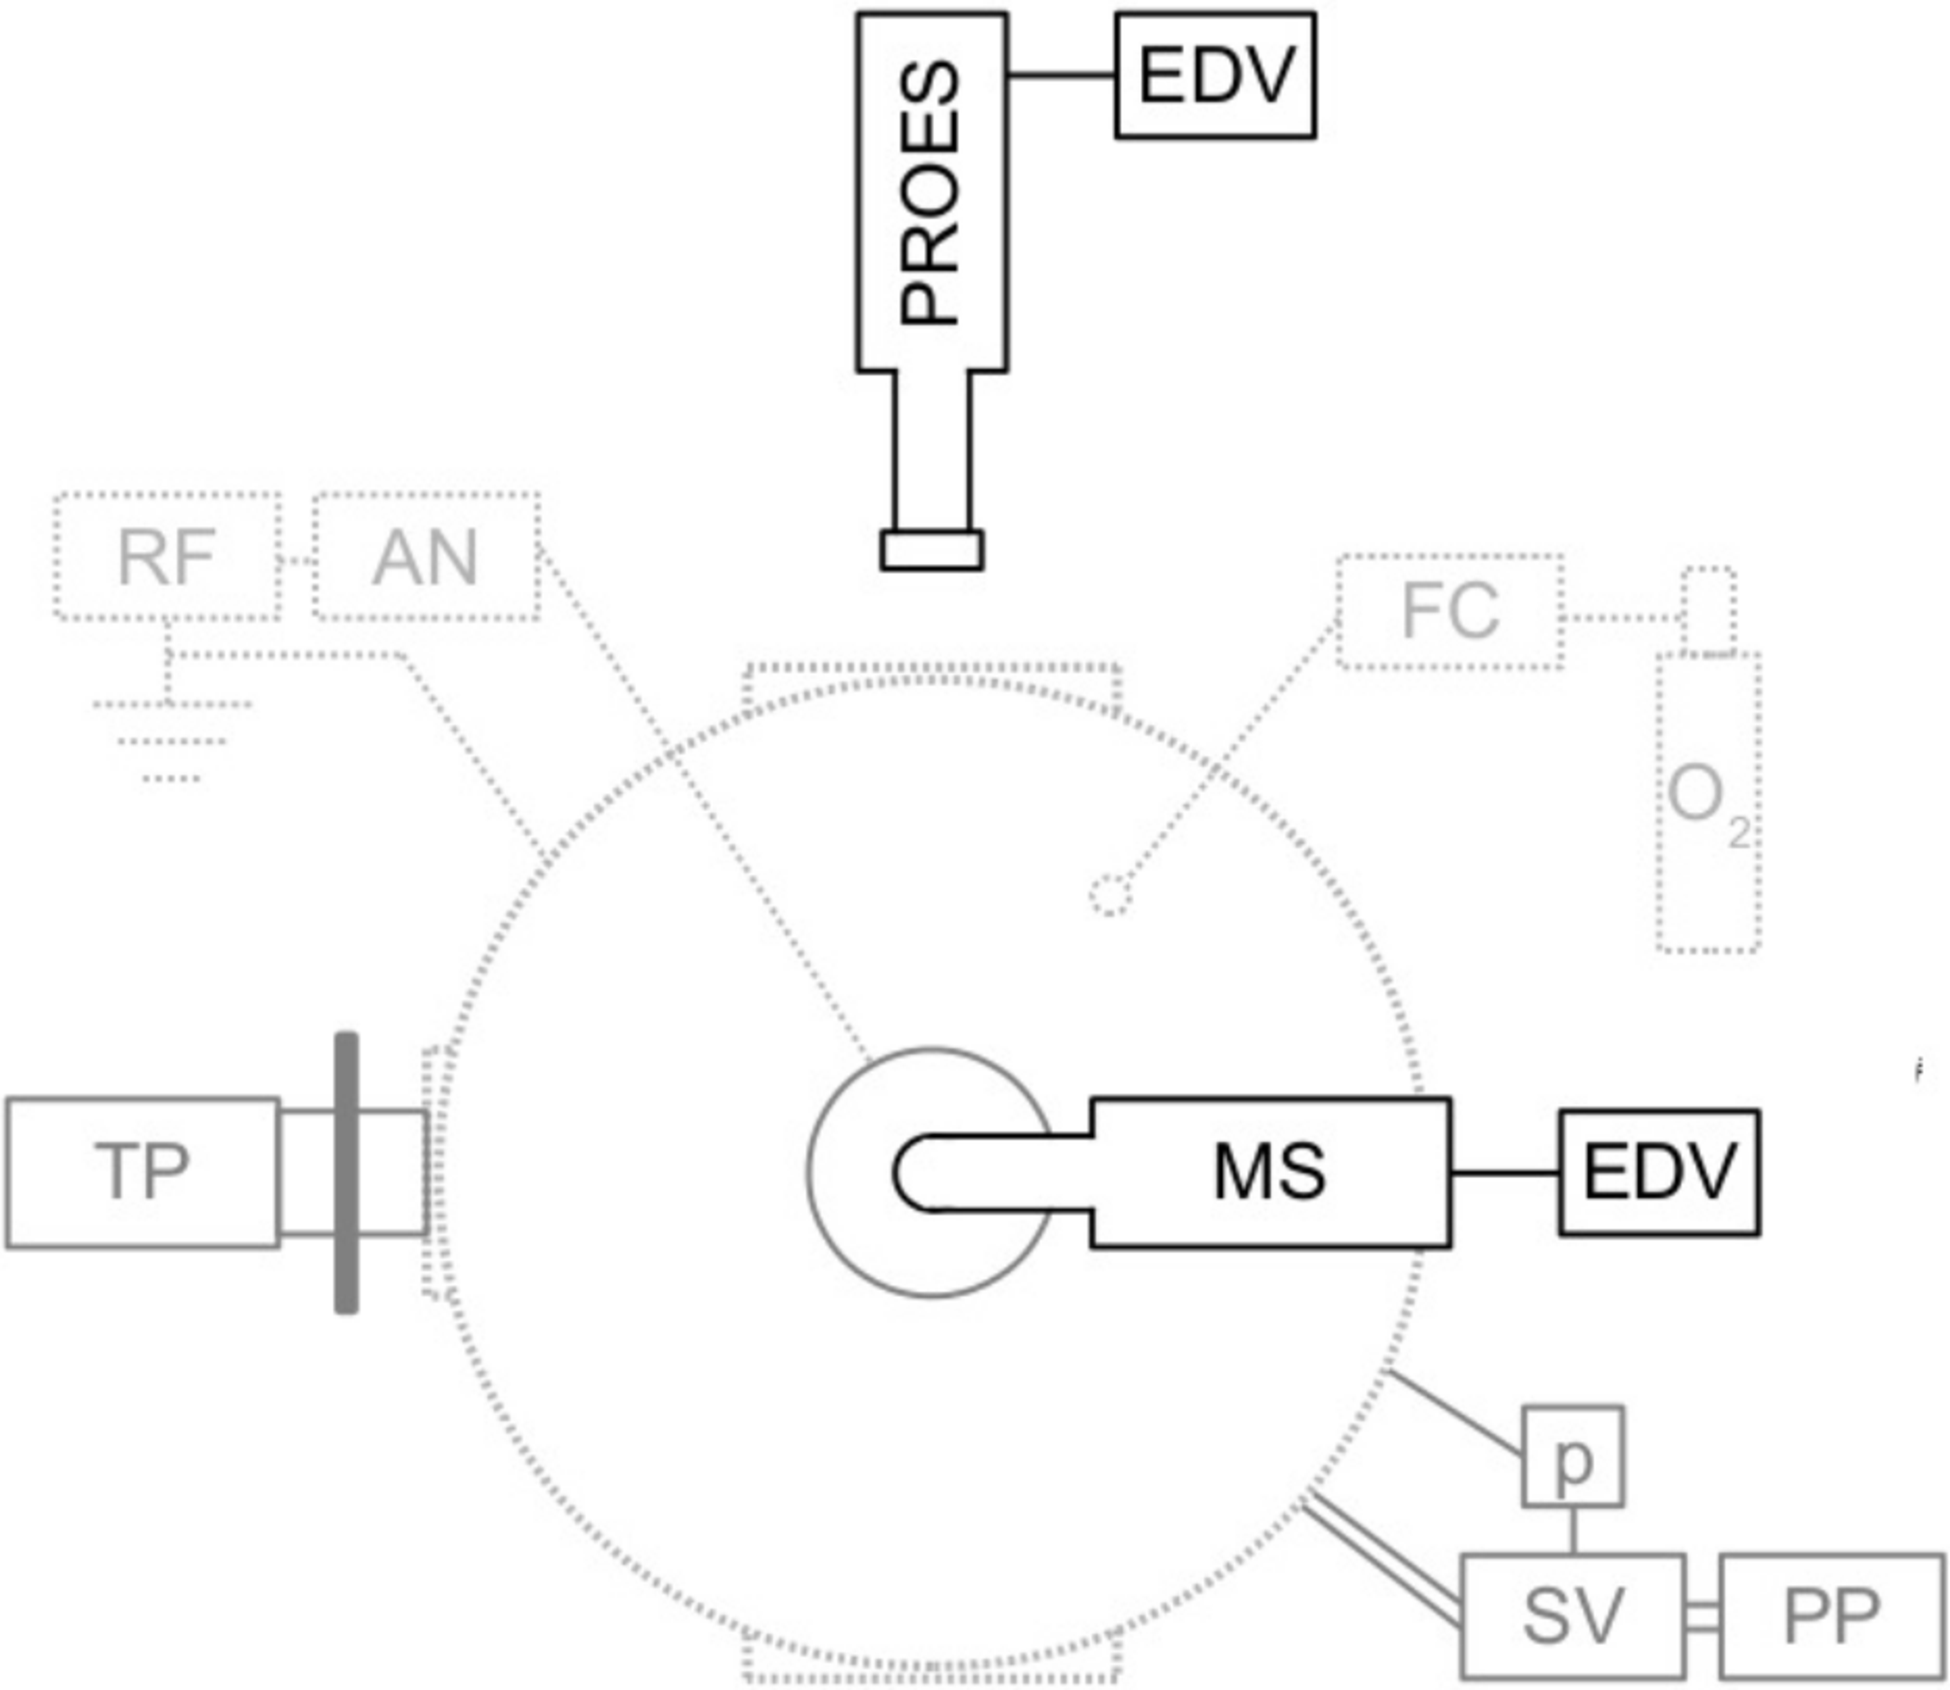
\includegraphics[width=0.5\textwidth]{figures/chamber_exp.pdf}
				\caption{%
					Top-down view schematic of the experiment~\cite{Scheuer15},~\cite{Kullig12}. Shown is the setup without microwave interferometer, like it was used by Küllig et al.}\label{fig:discharge_chamber}
			\end{figure}
%
			Here, the referenced experiment was used by Küllig et al.~\cite{Kullig12} and Scheuer~\cite{Scheuer15}, and consists of a cylindrical setup, filled with oxygen at low pressures and gas flow rates (see~\autoref{fig:discharge_chamber}). The stainless steel vacuum chamber had a diameter and height of $\unit[40]{cm}$ respectively and was filled with the process gas oxygen (O$\ix{2}$) at $\unit[5]{sccm}$ (\fett{FC}). The discharge configuration consisted of an electrode in the center with $\unit[10]{cm}$ of diameter and a rf generator, constantly operating at a frequency of $\unit[13,56]{MHz}$ and power outputs between $5$ and $\unit[150]{W}$ (\fett{RF} and \fett{AN}), leading to applied voltages in the range of $100$--$\unit[1500]{V}$. Shielding and discharge enclosure/chamber walls were grounded, therefore yielding a large area ratio between driven and grounded electrode and establishing a heavily asymmetric plasma. In addition, the powered electrode was coupled capacitively with the external generator, emphasizing the effect of the, in~\autoref{sec:selfbias} introduced self bias voltage. The value of $U\ix{sb}$ ranged, depending on power output and discharge pressure, from $-100$ up to $\unit[500]{V}$. In~\cite{Kullig12} the experiment was pulsed with short discharges at a frequency of $\unit[10]{Hz}$.	Line integrated measurements resulted in an average electron density of around $\tenpo{11}$--$\unit[\tenpo{12}]{cm^{-3}}$. Showing a schematic top-down view of the experiment is~\autoref{fig:discharge_chamber}. Here, the large ratio between driven and grounded parts is very well visualized. Hence, in later simulations it will be of sufficient accuracy to restrain the virtualized volume to a smaller setup.\\
			The figure below includes further diagnostics like a mass spectrometer (\fett{MS}) and phase resolved optical emission spectroscopy (\fett{PROES}). The latter measured the mentioned densities via line integration across the plasma volume. The MS is a key instrument for the investigation pursued in this thesis, as it also measures species counts with respect to their contribution to their correspoding energy distribution function. For example, the ions created via secondary processes in the discharge sheath are accelerated towards the bulk and thus get into the MS with their characteristic speeds and mass. A significant increase of electron density was found for rf powers larger than $\unit[50]{W}$ or $\unit[-220]{V}$ self bias voltage~\cite{Kullig12}. This led to a correlating negativ oxygen ion density reduction and decrease of the electronegativity ratio $\overline{n}_{i,-}/\overline{n}\ix{e}$ from $4$ to $0,03$. During a different operation mode --- called $\alpha$-mode, contrary to the afore-mentioned $\gamma$-mode --- at less than $\unit[50]{V}$ output power, electronegativity rises again, as well as the electron temperature $T\ix{e}$, yielding higher rate coefficients for, e.g.\@ dissociative electron attachment and the alike. See~\autoref{sec:anionproduction} for a more detailed approach.
%
		\subsection{Simulated Discharge}\label{sec:simulatedd_dis}
%
			All of the above conditions are sufficient for a practical approach at a labratory ccrf discharge with great repeatability. Though being highly optimized and developed over the course of many years, the twodimensional particle-in-cell code outlined above does not provide the tools and performance to feasibly simulate such large areas and particle numbers. Hence, one will reside to reducing the numerical expense by virtualizing smaller discharge areas and average densities, while trying to satisfy the same physical processes exhibited in~\cite{Kullig12}.\\
			The afore-mentioned 2d3v PIC code is used to simulated the referenced experiment. The spatial dimensions will be the radial component $r$ and axial coordinate $z$. The geometry and simulation is optimized for cylindrically symmetric gas discharges.\\
			To represent the strong asymmetry between driven and grounded wall areas, the sizes of anode, cathode and grounded chamber parts have been chosing accordingly. The experimental values for the self bias voltage $U\ix{sb}$ were used to create a dc offset on-top of the rf voltage $U\ix{rf}$ at the cathode. The domain composition with cells of width $\lambda\ix{D,e}/2$ (see~\autoref{sec:picbasics}) makes it even more difficult to appropriately model the system. Hence a smaller discharge volume of a $\unit[4,5]{cm}$ radius and an electrode gap of $\unit[2,5]{cm}$ will be simulated. This usually leads to cell counts up to $2\cdot\tenpo{5}$, which is small in comparison to the `real' experiment, which would have to be covered by over $\tenpo{6}$ cells. Furthermore, the numerical expense grows with $N\log(N)$, and $N$ being the particle number inside the cells (see~\autoref{sec:picsimulationmcc}).\\
			One has chosen pressures between $\unit[2]{Pa}$ and $\unit[10]{Pa}$, with the possibility of changing it later during the discharges simulation --- e.g\@ to change the bulk volume and densities. The secondary ion emission efficiency was set to $\eta=0,03$ in all cases, yielding a stable plasma sheath and hence SIE current into the bulk. In addition, a constant self bias of $\unit[-200]{V}$ was appplied at the cathode. The radio frequency was set to $\unit[13,56]{MHz}$.\\
			The governing electron density and temperature were set to $\unit[5\cdot\tenpo{9}]{cm^{-3}}$ and $\unit[5]{eV}$ respectively, which, as an initial value and property for scale, is sufficient for the necessary rate coefficients mentioned above. This led to the following important scales of simulation: 
%
			\begin{align}
				\lambda\ix{D}&=\unit[0,0235]{cm}\,,%
				\hspace*{2.0cm}%
				\omega\ix{p,e}=\unit[3,99\cdot\tenpo{9}]{Hz}%
				\label{equ:debyeandomega}\\[0.0cm]
				\Rightarrow \Delta x&=\frac{1}{2}\,\lambda\ix{D}=\unit[0,01174]{cm}\,,%
				\quad\quad%
				\Delta t=0,2\cdot\omega\ix{p,e}=\unit[5,015\cdot\tenpo{-11}]{s}%
				\label{equ:simulationscales}
			\end{align}
%			
			Thus a single rf cycle at the given frequency takes $1470$ steps, and the domain measures $384$ and $213$ in radial and axial dimension respectively. An ion temperature is adjusted via the fraction $T\ix{i}/T\ix{e}=0,008$, hence the corresponding velocities for the previously defined electron temperature $T\ix{e}=\unit[5]{eV}=\unit[5,8\cdot\tenpo{4}]{K}$ are found to be
%
			\begin{align}
				v\ix{th,e}=&\,\unit[9,37\cdot\tenpo{5}]{\frac{m}{s}}\,,%
				\quad\quad%
				c\ix{s,e}=\,\unit[3,87\cdot\tenpo{3}]{\frac{m}{s}}%
				\label{equ:electronvelocities}\\[0.0cm]%
%				IONS 
				v\ix{th,i}=&\,\unit[558,38]{\frac{m}{s}}\,,%
				\hspace*{1.2cm}%
				c\ix{s,i}=\,\unit[371,44]{\frac{m}{s}}%
				\label{equ:ionvelocities}
			\end{align}
%
		\begin{wrapfigure}{r}{0.3\textwidth}
			\centering
			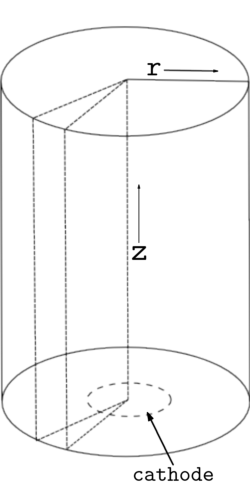
\includegraphics[width=0.275\textwidth]{figures/radial_cylinder.pdf}\\
			\vspace*{0.3cm}\hspace*{0.1cm}
			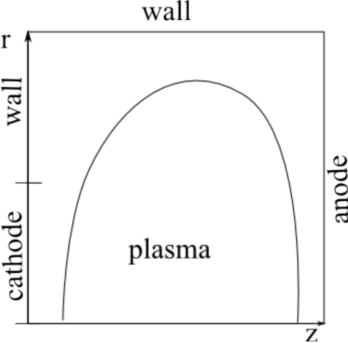
\includegraphics[width=0.275\textwidth]{figures/domain_slice.pdf}
			\caption{%
				Simplified cylinder schematic for the simulated experiment. The slice depicte in the top is shown below. There, boundaries and bulk position are outlined.}\label{fig:radialcylinder}
		\end{wrapfigure}
%
			Here, a single millisecond of operation takes days, if not weeks to simulate with a given timestep, like in~\autoref{equ:simulationscales}. Due to this and the fact, that the unit cell volume increases with the layer index of the radial coordinate --- one has to keep in mind that the cylindrical geometry is key to the simulation because important simplifications and assumptions inside the code itself are made uppon that premise ---, each particle carries an additional statistical weight. For example, a virtual neutral gas molecule of O$\ix{2}$ may represents up to $\tenpo{8}$ `real' particles in a laboratory plasma. This saves a vast amount of computational time by immensely reducing the particle counts necessary to sufficiently model the investigated physical processes. In this case, a single neutral gas particle is statistically amplified by a factor of $\approx 9,3\cdot\tenpo{7}$ to account for the gas density at $\unit[5]{Pa}$ and $\approx\unit[300]{K}$. This number is crucial to all collisional processes, where the molecular species O$\ix{2}$ is involved. Charged particle species share a common number amplification of $8489$. On top of both super particle factors, a scaling $\sim 1/r$ is applied to consider the variable cell volume.\\
			Another numerical tool is a constant neutral gas background. In the afore-metioned experiment, a working gas reservoir and flow rate meter control the pressure and exchange of O$\ix{2}$ inside the chamber. Due to the slow transition velocities of the cold neutral species, a working gas current from e.g.\@ behind an electrode is not feasible in this simulation. Collision rates and reaction coefficients are destroying neutral gas particles faster than they can be sufficiently supplied to the discharge. Hence, the O$\ix{2}$ molecules are initiated at time $t=0$ of the simulation --- this is done with respect to pressure, super particle factor and the alike ---, and are afterwards not altered in number or location. Though collision routines are still exercised, the corresponding push of the neutral species is skipped.
%
	\section{Simulated ccrf Oxygen Discharge}\label{sec:twod_secondaryions}
%
	In the collection of~\autoref{fig:2d-collection} twodimensional densities and potential are shown. Again, parameters were chosen as $U\ix{rf}=\unit[400]{V}$, $p=\unit[5]{Pa}$ and the initial species attributes to be $T\ix{e}=\unit[5]{eV}$, $n\ix{e,0}=\unit[5\cdot\tenpo{9}]{cm^{-3}}$ and $T\ix{i}/T\ix{e}=0,008$ respectively. 
%  
	\section{Anion Energy Distributions in Oxygen}\label{sec:twod_negionsdist}
%

% END
	%
\chapter{Conclusion}\label{sec:chapter_conclusion}
%

	%\chapter{Epilogue}

	\section{Local electrostratic field solver}

  \section{Diagnostics of current and charge}
  
  \section{Field calculation}

  \section{Comparison with Poisson-based solvers}

% ************************************************************************** %
%	
% ************************************************************************** %
% APPENDICES
	\appendix % Cue to tell LaTeX that following "chapters" are Appendices
	% Include the appendices of the thesis as separate files
	% Uncomment the lines as you write the Appendices
	\chapter{Appendix}
%
% ************************************************************************** %
% PHYSICAL PROPERTIES
  \section{Physical Properties}
  \begin{longtable}{m{0.32\textwidth}m{0.32\textwidth}m{0.32\textwidth}}
    \toprule
    \bfseries quantity & \bfseries equation & \bfseries relevance \\%
    \toprule\midrule\endhead%
      Debye length &%
        $\begin{aligned}
          \lambda\ix{D,j}^2&=\frac{\varepsilon\ix{0}k\ix{B}T\ix{j}}{n\ix{j}e^2} \\
          \lambda\ix{D}^2&={\left(\lambda\ix{D,e}^{-2}+\lambda\ix{D,i}^{-2}\right)}^{-1}
        \end{aligned}$ &%
          distance around a charge, at which quasi-neutrality is satisfied, %
          $\lambda\ix{D}$ is the combined screening length from individual species \\ \midrule%
      plasma parameter &%
        $\begin{aligned}
          N\ix{D} = n\frac{4}{3}\pi\lambda\ix{D}^{3}
        \end{aligned}$ &%
        number of particles inside Debye sphere, if $N\ix{D} \gg 1$ an ionized gas %
        is considered a plasma (degree of ionization) \\ \midrule%
      plasma frequency &%
        $\begin{aligned}
          \omega\ix{p,j}^2=\frac{n\ix{j}e^2}{\varepsilon\ix{0}m\ix{j}}=%
          \frac{v\ix{th,j}}{\lambda\ix{D,j}}=\frac{1}{\tau\ix{j}}
        \end{aligned}$ &%
          upper limit for interaction with fields/forces or external excitations %
          inverse screening time \\ \midrule%
      thermal velocity &%
        $\begin{aligned}
          v\ix{th,j}^2=\frac{k\ix{B}T\ix{j}}{m\ix{j}}
        \end{aligned}$ &%
          mean velocity from kinetic theory of gases \\ \midrule%
      coulomb logarithm &%
        $\begin{aligned}
          &\ln\left(\Lambda\right) \\ \\
          &\Lambda=\frac{b\max}{b\min}= \\ \\
          &\lambda\ix{D}\cdot%
          \frac{4\pi\varepsilon\ix{0}\mu v\ix{th}^{2}}{e^{2}} 
        \end{aligned}$ &%
          dimensionless scale for transport processes inside discharge \newline
          fraction of probability for a cumulative $90^{\circ}$ scattering by many small %
          pertubation collisions and a single right angle scattering \\ \midrule%
      collision frequency &%
        $\begin{aligned}
          \nu\ix{j}=\frac{e^{4}n\ix{j}\ln\left(\Lambda\right)}%
          {8\sqrt{2m\ix{j}}\pi\varepsilon\ix{0}{\left(k\ix{B}T\ix{j}\right)}^{3/2}}
        \end{aligned}$ &%
          two body coulomb collision frequency inside species j \\ \midrule%
      particle distance \& \newline mean free path &%
        $\begin{aligned}
          &\overline{b}=\frac{\hbar}{m\ix{j}v\ix{th,j}} \\ \\
          &s\ix{mfp,j}=\frac{v\ix{th,j}}{\nu\ix{j,k}}
        \end{aligned}$ &%
          mean inter particle distance for species j \newline% 
          free flight between subsequent collisions of species j and k %
          with collision frequency $\nu\ix{j,k}$ \\ \midrule%
      speed of sound &%
        $\begin{aligned}
          c\ix{S}^{2}&=\frac{\gamma Zk\ix{B}T\ix{e}}{m\ix{i}} \\
          \gamma&=1+2/f=5/3
        \end{aligned}$ &%
        speed of longitudinal ion waves at electron pressure \newline%
        adiabatic coefficient with f, the kinetic degree of freedom\\ \midrule%
      Debye-Hückel potential &%
        $\begin{aligned}
          \Phi=\frac{Q}{4\pi\varepsilon|\vec{r}|}%
          \euler^{-\frac{|\vec{r}|}{\lambda\ix{D}}}
        \end{aligned}$ &%
        electrostatic potential of charge particle $Q$ at distance $|\vec{r}|$, \newline%
        equal to coulomb interaction with additional%
        shielding by charged particles \\ \midrule%
      drift velocity &
        $\begin{aligned}
          v\ix{d,j}=u\ix{j}=\frac{j\ix{j}}{n\ix{j}q}=\frac{m\sigma E}{\rho ef}
        \end{aligned}$ &%
        average velocity of a particle in a conductor with an electric field applied E, \newline%
        where $N$ is the number of free electrons per atom \\%
      electric mobility &
        $\begin{aligned}
          \mu\ix{j}=\frac{v\ix{d}}{E}
        \end{aligned}$ &%
        ability of charged particle of moving through an electric field \\%
    \midrule\bottomrule%
    \caption[Selection of physical properties of a low temperature ccrf discharge]{%
      Selection of physical properties of a low temperature ccrf discharge. The index $j$ denotes the %
      species, e.g.\@ electrons, ions. Used quantities can be found in the preface %
      in~\autoref{tabe:physicalconstants}.}\label{tabe:physicalquantities}
  \end{longtable}
% ************************************************************************** %
%   
		\clearpage
    \section[Energy Distributions from 2D PIC]%
            {Simulated Energy Distribution\\
            Functions from 2D PIC}\label{sec:appendix_results}
%
        \begin{center}
            \begin{figure}[!h]
                \centering
                \begin{subfigure}{0.49\textwidth}
									\includegraphics[height=0.3\textheight]%
                        {figures/results/2D/44332/e_dens.png}
                \end{subfigure}
                \begin{subfigure}{0.49\textwidth}
									\includegraphics[height=0.3\textheight]%
                        {figures/results/2D/44426/e_dens.png}
                \end{subfigure}
                %\caption[2D electron and ion density]{%
                %    Electron density from the two previously %
								%		described asymmetric 2D simulations.}
                %\label{fig:app_dens}
            %\end{figure}
						%\begin{figure}
								%\centering
                \begin{subfigure}{0.49\textwidth}
									\includegraphics[height=0.3\textheight]%
                        {figures/results/2D/44332/ni_dens.png}
                \end{subfigure}
                \begin{subfigure}{0.49\textwidth}
									\includegraphics[height=0.3\textheight]%
                        {figures/results/2D/44426/ni_dens.png}
                \end{subfigure}
								\newline
                %\caption[2D electron and ion density]{%
                %    Negative ion density from the two previously %
								%		described asymmetric 2D simulations.}
                %\label{fig:app_dens_ni}
            %\end{figure}
						%\begin{figure}[!b]
                %\centering
                \begin{subfigure}{0.49\textwidth}
									\includegraphics[height=0.22\textheight]%
                        {figures/results/2D/44332/e_distz.png}
                \end{subfigure}
                \begin{subfigure}{0.49\textwidth}
									\includegraphics[height=0.22\textheight]%
                        {figures/results/2D/44426/e_distz.png}
                \end{subfigure}
               	\caption[Electron and negative ion panel]{%
									\fett{Top}: electron density, \fett{Mid}: negative ion density, %
									\fett{Bottom}: axial compontent of electron EDF from a 2D simulation %
										of the two asymmetrical discharges discussed before-hand.}
                \label{fig:app_dens}
            \end{figure}
						\clearpage
            \begin{figure}
                \centering
                \begin{subfigure}{0.49\textwidth}
                    \includegraphics[width=1.0\textwidth]%
                        {figures/results/2D/44332/i_distz.png}
                \end{subfigure}
                \begin{subfigure}{0.49\textwidth}
                    \includegraphics[width=1.0\textwidth]%
                        {figures/results/2D/44426/i_distz.png}
                \end{subfigure}
                \caption[Axial ion EDF from 2D]{%
                    Axial compontent of ion EDF from a 2D simulation %
										of the two asymmetrical discharges discussed before-hand.}
                \label{fig:app_edf_i}
            \end{figure}
						\vfill
            \begin{figure}
                \centering
                \begin{subfigure}{0.49\textwidth}
                    \includegraphics[width=1.0\textwidth]%
                        {figures/results/2D/44332/ni_distz.png}
                \end{subfigure}
                \begin{subfigure}{0.49\textwidth}
                    \includegraphics[width=1.0\textwidth]%
                        {figures/results/2D/44426/ni_distz.png}
                \end{subfigure}
                \caption[Axial negative ion EDF from 2D]{%
                    Axial compontent of negative ion EDF from a 2D simulation %
										of the two asymmetrical discharges discussed before-hand.}
                \label{fig:app_edf_ni}
            \end{figure}
        \end{center}
%
		\clearpage
    \listoffigures % Prints the list of figures
	\listoftables % Prints the list of tables

% ************************************************************************** %
%
% ************************************************************************** %
% BIBLIOGRAPHY
	\printbibliography[heading=bibintoc]
% ************************************************************************** %
% END OF DOCUMENT
\end{document}  
% test bibliography for completion
\bibliography{master_thesis.bib}
